\documentclass[12pt,a4paper]{article}

% Language setting
% Replace `english' with e.g. `spanish' to change the document language
\usepackage[english]{babel}

% Set page size and margins
% Replace `letterpaper' with `a4paper' for UK/EU standard size
\usepackage[letterpaper,top=2cm,bottom=2cm,left=3cm,right=3cm,marginparwidth=1.75cm]{geometry}
\usepackage{amsthm}
\usepackage{subcaption}
\newtheorem{definition}{Definition}
% Useful packages
\usepackage{amsmath}
\usepackage{graphicx}
\usepackage[colorlinks=true, allcolors=blue]{hyperref}
\usepackage{graphicx}   % For including images
\usepackage{caption}    % For captions
\usepackage{float}      % To control figure placement
\usepackage{lipsum}     % For placeholder text (optional)
\usepackage{hyperref}
\usepackage{setspace}

\usepackage{mathtools}
\usepackage[utf8]{inputenc}
\usepackage{listings}
\usepackage{color}

\definecolor{codegreen}{rgb}{0,0.6,0}
\definecolor{codegray}{rgb}{0.5,0.5,0.5}
\definecolor{codepurple}{rgb}{0.58,0,0.82}
\definecolor{backcolour}{rgb}{0.95,0.95,0.92}

\lstdefinestyle{mystyle}{
    backgroundcolor=\color{backcolour},   
    commentstyle=\color{codegreen},
    keywordstyle=\color{magenta},
    numberstyle=\tiny\color{codegray},
    stringstyle=\color{codepurple},
    basicstyle=\ttfamily\footnotesize,
    breakatwhitespace=false,         
    breaklines=true,                 
    captionpos=b,                    
    keepspaces=true,                 
    numbers=left,                    
    numbersep=5pt,                  
    showspaces=false,                
    showstringspaces=false,
    showtabs=false,                  
    tabsize=2
}

\lstset{style=mystyle}

\usepackage{tikz}
\usetikzlibrary{shapes.geometric, arrows}

\usepackage{tikz}
\usetikzlibrary{shapes.geometric, arrows}

\tikzstyle{block} = [rectangle, rounded corners, minimum width=3cm, minimum height=1cm,text centered, draw=black, fill=blue!30]
\tikzstyle{arrow} = [thick,->,>=stealth]
\tikzstyle{decision} = [diamond, minimum width=2cm, minimum height=2cm, text centered, draw=black, fill=green!30]


\tikzstyle{startstop} = [rectangle, rounded corners, minimum width=3cm, minimum height=1cm,text centered, draw=black, fill=white!30]
\tikzstyle{process} = [rectangle, minimum width=3cm, minimum height=1cm, text centered, draw=black, fill=white!30]
\tikzstyle{arrow} = [thick,->,>=stealth]

%\title{Your Paper}
%\author{You}
\linespread{1.15}
\begin{document}

\pagenumbering{}

\newpage
\begin{center}
    \section*{ABSTRACT}
\end{center}
\hspace{1em}This study aims to predict the age group most vulnerable to diabetes in the context of emerging viral threats. We employ and compare two decision-making techniques: Simple Additive Weighting (SAW) and Fuzzy Multiple Criteria Decision Making (MCDM) using the Technique for Order of Preference by Similarity to Ideal Solution (TOPSIS). Real time data on age, glucose levels, blood pressure, skin thickness, insulin, body mass index and diabetes pedigree function are collected to identify susceptible individuals. The research evaluates the effectiveness of both techniques and recommends the most suitable approach for prediction. Finally, the study offers recommendations for diabetes management based on the finding.

\newpage
% Create the table of contents
\tableofcontents
\newpage
\pagenumbering{arabic}
\begin{center}
    \section*{CHAPTER-I}
    %\section{INTRODUCTION}
\end{center}
\section{INTRODUCTION}
\hspace{3em}Fuzzy Logic, a concept introduced by Lotfi Zadeh in 1965, extends classical logic to handle the concept of partial truth—where the truth value may range between completely true and completely false. Unlike binary logic, which restricts expressions to strict yes or no values, fuzzy logic allows for a more flexible approach by accommodating varying degrees of truth. This makes it particularly useful for dealing with uncertainties and imprecise information, especially in decision-making processes.\\

MCDM is a branch of decision science that involves evaluating and ranking multiple alternatives based on a set of criteria. In real-world scenarios, decision-making often requires considering various conflicting criteria, and MCDM provides systematic methods to address this complexity. By using MCDM techniques, decision-makers can make informed and rational choices in situations where multiple factors need to be considered, such as resource allocation, project selection, and strategic planning.\\

One of the simplest and most commonly used MCDM methods is the SAW method. SAW is based on the principle of weighted summation, where each criterion is assigned a weight reflecting its importance. The method evaluates each alternative by calculating the weighted sum of its scores across all criteria. SAW is popular due to its simplicity and ease of implementation, making it a preferred choice for preliminary decision-making tasks.\\

By combining fuzzy logic with MCDM approaches like SAW, decision-makers can handle the inherent uncertainties in evaluating and ranking alternatives. This fusion allows for more robust and adaptable solutions in complex, real-world scenarios where precise data may not always be available.

\subsection{PRELIMINARIES}
\subsubsection*{MCDM [9]}
\hspace{1em}It refers to a set of methods and processes used to evaluate and prioritize alternatives based on multiple, often conflicting, criteria. MCDM helps decision-makers identify the most suitable option among a set of alternatives by considering various factors simultaneously.


\subsubsection*{SAW IN MCDM [9]}
\hspace{1em}It is a straightforward MCDM method
used to evaluate and rank alternatives based on multiple criteria. It
involves scoring each alternative on each criterion, then aggregating
these scores using a weighted sum to produce an overall score for each
alternative.

\subsubsection*{DECISION MATRIX [9]}
\begin{enumerate}
\item\textbf{Define the Decision Matrix:} Let m be the number of alternatives and $n$ be the number of criteria. The decision matrix $D$ is defined as:
\[
D=
\begin{bmatrix}
a_{11} & a_{12} &\cdots & a_{1n}\\
a_{21} & a_{22} &\cdots & a_{2n}\\
\vdots & \vdots & \ddots & \vdots\\
a_{m1} & a_{m2} &\cdots & a_{mn}\\
\end{bmatrix}
\]
where $a_{ij}$represents the performance of alternative $i$ on criterion $j$.\\
\item\textbf{Normalize the Decision Matrix:} Normalize the matrix to bring all criteria to a comparable scale. For beneficial criteria, the normalization can be done as:
\begin{equation*}
      r_{ij}=\frac{a_{ij}}{max(a_{j})}      
\end{equation*}
For non-beneficial criteria, it can be:
\begin{equation*}
      r_{ij}=\frac{min(a_{j})}{a_{ij}}  
\end{equation*}

\item\textbf{Weight the Normalized Values:} Let $w_{j}$ be the weight assigned to criterion $j$ \\(where $\sum\limits^{n}_{j=1}w_{j}=1 $) the weighted normalized score is calculated as:
\begin{equation*}
    v_{i}=\sum\limits^{n}_{j=1}w_{j}.r_{ij}
\end{equation*}

\item\textbf{Rank the Alternatives:} Finally, rank the alternatives based on their scores. The alternative with the highest score is considered the best option.
\end{enumerate}



\subsubsection*{FUZZY SET [9] }
\hspace{1em}A fuzzy set is defined by a membership function $\mu_{a}(x)$, which assigns a degree of membership to each element $x$. This value ranges between 0 and 1:

\begin{center}  
   $ \mu_{a}(x)$=\text{degree of membership of $x$ in set $A$ }
\end{center}

\subsubsection*{MEMBERSHIP FUNCTION [9] }
\hspace{1em}Common types of membership functions include:

\begin{itemize}
    \item Triangular :$\mu_{A}(x)=max(0,\frac{z-a}{b-a},\frac{c-x}{c-b})$

    \item Trapezoidal, Gaussian, etc
\end{itemize}

\subsubsection*{FUZZY RULES [9]}
\hspace{1em} Fuzzy rules are expressed in the form of "If-Then" statements. For example:

\begin{itemize}
    \item \textbf{Rule 1:} If the temperature is "high," then the fan speed is "fast."

    \item \textbf{Rule 2:} If the temperature is "medium," then the fan speed is "medium."
\end{itemize}

\subsubsection*{FUZZY INFERENCE [9]}
\hspace{1em}Fuzzy inference combines fuzzy rules to determine the output based on input values. The most common methods are:
\begin{itemize}
    \item 	\textbf{Mamdani:} Uses fuzzy sets for both inputs and outputs.

    \item \textbf{Sugeno:} Uses fuzzy sets for inputs and crisp functions for outputs.
\end{itemize}


\textbf{Example}
\textbf{Scenario:} Determine fan speed based on temperature.

\begin{itemize}
    \item \textbf{Input Temperature:} 30°C

    \item \textbf{Fuzzy Sets:}
    \begin{itemize}
        \item Low: $\mu_{Low}(30)=0.1$ 

        \item Medium: $\mu_{Medium}(30)=0.7$

        \item High: $\mu_{High}(30)=0.2$
        
    \end{itemize}
\item \textbf{Fuzzy Rules:}
\begin{itemize}
    \item If temperature is Low, then fan speed is Slow.
   
    \item  If temperature is Medium, then fan speed is Medium.

    \item If temperature is High, then fan speed is Fast.
    
\end{itemize}
    
\end{itemize}

\subsubsection*{Decision making:}
\begin{enumerate}
    \item \textbf{Fuzzification: }Convert the crisp input into fuzzy values using the membership functions.

    \item \textbf{Rule Evaluation:} Apply fuzzy rules to determine the degrees of output based on the input fuzzy values. For instance:

    \begin{itemize}
        \item Output for Rule 1:$\mu_{Slow}(30)=0.1$

        \item Output for Rule 2: $\mu_{Medium}(30)=0.7$

        \item Output for Rule 3: $\mu_{High}(30)=0.2$
        
    \end{itemize}

   \item \textbf{	Aggregation:}Combine the outputs from all rules. For instance, the overall output membership for fan speed might be: 
   \begin{equation*}
\mu_{Output}=max(\mu_{Slow},\mu_{Medium},\mu_{Fast})=max(0.1,0.7,0.2)=0.7
   \end{equation*}

   \item \textbf{	Defuzzification:} Convert the fuzzy output back into a crisp value using methods like the centroid method:\\
\begin{center}
   \text{ Fan Speed} = $\frac{(\mu_{i}.x_{i})}{\mu_{i}}$
\end{center}
\end{enumerate}
    
\subsubsection*{FUZZY NUMBERS [9]}

 \hspace{1em}A real fuzzy number $A$ is described as any fuzzy subset of the real line $R$ with membership function $f_{A}$ which possesses the following properties where a, b, c, and d are real numbers:

\begin{itemize}

    \item $f_{A}$ is a continuous mapping from $R$ to the closed interval $[0,1]$.

    \item $f_{A}(x) = 0$ , for all $x \in (-\infty , a]$. 
    \item $f_{A}$ is strictly increasing on $[a, b]$.

    \item $f_{A}(x) = 1$ , for all $x \in [b , c]$.
    \item $f_{A}$ is strictly decreasing on $[c, d]$.

    \item $f_{A}(x) = 0$ , for all $x \in [d , \infty )$.
    
\end{itemize}
\hspace{1em}We may let $a = -\infty$ , or $a = b$, or $b =  c$, or $c = d$, or $d = +\infty$. Unless elsewhere specified, it is assumed that $A$ is
convex, normal and bounded, i.e. $-\infty < a, d < +\infty$.[1]
The membership function $f_{A}$ of the fuzzy number $A$ can also
be expressed as:


\[
f_A(x) =
\begin{cases} 
f^L_A(x) & \text{if } (a \leq x \leq b) \\
1 & \text{if } (b \leq x \leq c) \\
f^R_A(x) & \text{if } (c \leq x \leq d) \\
0 & \text{otherwise}
\end{cases}
\]

where $f^{L}_{A}(x)$ and $f^{R}_{A}(x)$ are the left and right membership functions of fuzzy number $A$, respectively\\
The fuzzy number $A$ is a triangular fuzzy number if its membership function $f_{A}$ is given by
\[
f_A(x) =
\begin{cases} 
\frac{(x - a)}{(b - a)} & \text{if } a \leq x \leq b \\
\frac{(x - c)}{(b - c)} & \text{if } b \leq x \leq c \\
0 & \text{otherwise}
\end{cases}
\]

where a, b and c are real numbers.



\subsubsection*{TOPSIS [5]}
\hspace{1em}It is a MCDM method that identifies the best alternative based on the shortest distance to an ideal solution and the farthest distance from an anti-ideal solution. The fundamental principle behind TOPSIS is that the chosen alternative should have the closest proximity to the ideal solution while being the farthest from the worst-case scenario.

\subsubsection*{FUZZY TOPSIS IN MCDM [5]}
\hspace{1em}It is an extension of the traditional TOPSIS method that incorporates fuzzy logic to handle uncertainty and imprecision in decision-making. This approach is particularly useful when decision criteria are subjective or qualitative, allowing for a more detailed evaluation of alternatives.

\begin{enumerate}
    \item \textbf{Fuzzy Decision Matrix:} The fuzzy decision matrix D is represented as:
    \[
D=
\begin{bmatrix}
a_{11} & a_{12} &\cdots & a_{1n}\\
a_{21} & a_{22} &\cdots & a_{2n}\\
\vdots & \vdots & \ddots & \vdots\\
a_{m1} & a_{m2} &\cdots & a_{mn}\\
\end{bmatrix}
\]
where $a_{ij}$represents the performance of alternative $i$ on criterion $j$.\\

\item \textbf{Normalization:} The normalized fuzzy decision matrix can be calculated as:
\begin{eqnarray*}
    r_{ij}=\frac{a_{ij}}{\sqrt{\sum\limits^{m}_{i=1}a^{2}_{ij}}}
\end{eqnarray*}
\item \textbf{Weighted Normalized Decision Matrix:} The weighted normalized values are computed by multiplying each normalized value by the corresponding weight $w_{j}$:
\begin{equation*}
    v_{ij}=w_{j}.r_{ij}
\end{equation*}
\item \textbf{Ideal and Negative Ideal Solutions:} The positive ideal solution $A^{+}$ and negative ideal solution $A^{-}$ are defined as:
\begin{center}
    $A^{+}$={$max(v_{ij})$}\\
    $A^{-}$={$min(v_{ij})$}
\end{center}
\item \textbf{Separation Measures:} The separation from the ideal and negative ideal solutions are calculated as:
\begin{center}
   $S_{i}^{+}=\sqrt{\int^{n}_{j=1}(v_{ij}-A^{+})^{2}}$\\
   $S_{i}^{-}=\sqrt{\int^{n}_{j=1}(v_{ij}-A^{-})^{2}}$   
\end{center}
\item \textbf{Relative Closeness to the Ideal Solution:} The relative closeness of each alternative to the ideal solution is given by:
\begin{center}
 $C_{i}=\frac{S_{i}}{S_{i}+S_{j}}$   
\end{center}
    
\end{enumerate}
\subsection{BOOLEAN LOGIC - FUZZY LOGIC}

\hspace{1em}\textbf{Boolean Logic [21]: } It is a logic form of algebra where the values of the variables can only be true of false (1 or 0). It is based on binary values and uses logical operators such as AND, OR and NOT. The operations yield binary outcome, making it suitable for digital circuits and simple decision-making processes.\\
    
\textbf{Fuzzy Logic [21]:} It extends boolean logic by allowing for degrees of truth rather than a strict true/ false dichotomy. It uses membership functions to represent the degree to which a variable belongs to a set, allowing for a continuum of truth values ranging from 0 to 1. This makes fuzzy logic useful in situations where information is uncertain or imprecise.

\subsection{FUZZY LOGIC}
\hspace{1em}Fuzzy logic is a form of many-valued logic that deals with reasoning that is approximate rather than fixed and exact. Unlike classical Boolean logic, which works with binary values (true or false), fuzzy logic allows for degrees of truth, meaning values can range between 0 and 1 [23].\\

This approach is particularly useful for modeling complex systems where precise information is unavailable or where systems operate in a gray area rather than in black and white. Fuzzy logic uses fuzzy rules that incorporate degrees of membership. Concepts are expressed in terms of membership functions that define how much an element belongs to a fuzzy set. For example, fuzzy rules might include, “If the temperature is somewhat high, then the fan speed should be moderately high.” Fuzzy operators handle the combination of these rules. Fuzzy logic plays a significant role in decision-making, particularly in scenarios where information is imprecise, uncertain, or incomplete. It enhances decision-making by offering a flexible, human-like approach to handling uncertainty and imprecision. Its ability to model complex, real-world scenarios with degrees of membership and rule-based reasoning makes it a powerful tool in a wide range of applications. Whether improving system performance, facilitating complex multi-criteria decisions, or enhancing user interaction, fuzzy logic significantly contributes to more effective and nuanced decision-making processes. This understanding of fuzzy logic’s role in decision-making can be applied to various projects and industries, leveraging its strengths to address challenges and improve outcomes. In fuzzy logic, the concepts of black, white, and gray areas represent the spectrum of truth values:
\begin{itemize}

\item\textbf{Black Area (True/Yes):} This represents absolute truth, where a statement is completely true. For example, "The temperature is hot" might fall into this category if the temperature exceeds a specific threshold.
\item\textbf{White Area (False/No):} This indicates absolute falsehood, where a statement is completely false. For instance, "The temperature is cold" might be in this area if the temperature is well above freezing.
\item\textbf{Gray Area (Partial Truth):} This encompasses the range of values between true and false, where statements can be partially true or false. For example, "The temperature is warm" can have varying degrees of truth, depending on the context (e.g., 20°C might be considered warm by some but cool by others).

\end{itemize}



\subsection{BASICS OF MATLAB}

\hspace{2em}MATLAB [20] - "Matrix Laboratory," is a high-level programming language and interactive environment designed primarily for numerical computing, data analysis, and visualization. Developed by MathWorks, MATLAB is widely used in engineering, scientific research, and academia for its powerful computational capabilities and ease of use.\\

\hspace{1em}MATLAB is defined as a software platform that provides an integrated environment for algorithm development, data analysis, visualization, and numerical computation. Its core is based on matrices, making it particularly well-suited for tasks involving linear algebra, signal processing, control systems, and various other mathematical computations .

\subsubsection*{BASICS OF MATLAB}
\begin{enumerate}
    \item \textbf{Core Language:} MATLAB's syntax is designed to be intuitive and user-friendly, allowing users to write complex mathematical expressions with ease. Variables can be defined and manipulated in a straightforward manner, which facilitates rapid prototyping.

    \item \textbf{Matrices and Arrays:} At its core, MATLAB operates primarily on matrices and arrays, allowing for efficient manipulation of large data sets. Users can perform a variety of operations, such as addition, multiplication, and inversion, directly on these structures.

    \item \textbf{Built-in Functions:} MATLAB comes with a vast library of built-in functions for mathematical operations, statistical analysis, optimization, and more. This extensive collection enables users to implement complex algorithms without needing to code everything from scratch.

    \item \textbf{Data Visualization:} One of MATLAB's strengths lies in its ability to create high-quality graphical representations of data. Users can generate plots, charts, and visualizations with simple commands, making it easy to analyze and interpret results.

    \item \textbf{Toolboxes:} MATLAB offers numerous specialized toolboxes that extend its capabilities to specific domains such as signal processing, image processing, machine learning, and control systems. These toolboxes provide additional functions and tools tailored for particular applications.

    \item \textbf{Simulink:} A companion product to MATLAB, Simulink allows users to model, simulate, and analyze dynamic systems using a graphical interface. It is particularly useful for control system design and simulation.

    \item \textbf{Cross-Platform Compatibility:} MATLAB is available on various operating systems, including Windows, macOS, and Linux, which facilitates collaboration and sharing of MATLAB scripts across different environments. 
\end{enumerate}
\subsection{BASICS OF PYTHON}
     
     \hspace{2em}Python is an open-source, high-level programming language that has gained immense popularity due to its versatility, ease of learning, and extensive library support. Created by Guido van Rossum and first released in 1991, Python emphasizes readability and simplicity, making it an ideal choice for beginners and experienced developers alike. Its design philosophy encourages code readability, which is reflected in its use of significant indentation [14].

\subsubsection*{FEATURES}
\begin{enumerate}
    \item\textbf{Simple Syntax:} Python’s syntax closely resembles natural language, which allows developers to express concepts in fewer lines of code compared to languages like C++ or Java. This simplicity facilitates rapid application development and reduces the learning curve for new programmers.

\item\textbf{Interpreted Language:} As an interpreted language, Python executes code line-by-line, which aids in debugging and enhances flexibility during development. This feature allows developers to test small code snippets in real-time, making it easier to experiment and iterate.

\item\textbf{Dynamic Typing:} Python supports dynamic typing, meaning that variables do not require explicit declaration before they are used. This flexibility allows for quicker coding and reduces the overhead of type management.

\item\textbf{Extensive Libraries and Frameworks:} Python boasts a rich ecosystem of libraries and frameworks, such as NumPy for numerical computing, Pandas for data analysis, Flask and Django for web development, and TensorFlow and PyTorch for machine learning. These tools significantly accelerate development processes and enable developers to implement complex functionalities with ease.

\item\textbf{Cross-Platform Compatibility:} Python is a cross-platform language, which means that Python programs can run on various operating systems, including Windows, macOS, and Linux, without requiring modifications. This characteristic enhances its usability in diverse environments.
\end{enumerate}

Python is a powerful and flexible programming language that caters to a wide range of applications, from web development and data analysis to automation and artificial intelligence. Its simple syntax, extensive libraries, and supportive community make it an excellent choice for both new and seasoned developers. As technology continues to evolve, Python's relevance in the programming landscape is likely to grow, making it a valuable skill for anyone looking to thrive in the digital age. Whether you are building a simple script or developing complex systems, Python offers the tools and capabilities needed to bring your ideas to life.

\newpage
\begin{center}
    \section*{CHAPTER – II}
\end{center}


\section{LITERATURE REVIEW}

\subsection{HISTORY OF FUZZY}
\hspace{1em}In many real-world situations, information is not precise or binary (true or false). Instead, it is often vague, uncertain, or imprecise. Traditional logic and mathematics struggle to handle such complexity effectively.


\subsection*{Early Foundations}
\begin{itemize}

\item \textbf{Ancient and Philosophical Roots (Pre-$20^{th}$ Century):} The concept of vagueness and imprecision has roots in ancient philosophy. Philosophers such as Aristotle explored ideas related to degrees of truth and gradations of qualities, though these were not formalized into a structured theory.
\end{itemize}

\subsection*{The Birth of Fuzzy Logic}
\begin{itemize}

\item \textbf{1965: Lotfi Zadeh’s Groundbreaking Work:} The formal foundation of fuzzy logic was laid by Lotfi A. Zadeh, a professor of computer science and electrical engineering at the University of California, Berkeley. In his seminal paper titled "Fuzzy Sets," Zadeh introduced the concept of fuzzy sets, which extend classical set theory to handle partial membership. Unlike classical sets, where an element either belongs or does not belong to a set, fuzzy sets allow for degrees of membership.

\item \textbf{1966: Extension to Fuzzy Logic:} Following the introduction of fuzzy sets, Zadeh further developed fuzzy logic as a way to handle reasoning that is approximate rather than fixed and exact. This extension provided a framework to model human reasoning and decision-making processes that involve uncertainty and vagueness.
\end{itemize}

\subsection*{Early Applications and Development}
\begin{itemize}

\item \textbf{1970s: Initial Applications:} The initial applications of fuzzy logic were in control systems. Early adopters began to apply fuzzy logic to problems where binary logic and classical control systems struggled, such as in the automotive and aerospace industries. One notable early application was the development of fuzzy logic controllers for appliances, such as washing machines and air conditioners, enhancing their performance and efficiency.

\item \textbf{1980s: Expansion and Commercialization:} During the 1980s, fuzzy logic gained popularity and saw increased application in various fields. It was integrated into a variety of consumer products, including automotive systems (e.g., automatic transmission control) and industrial processes. This period also saw the emergence of commercial tools and software based on fuzzy logic, making it more accessible to engineers and researchers.

\end{itemize}

\subsection*{Modern Advancements}
\begin{itemize}

\item \textbf{1990s: Theoretical and Practical Advances:} The 1990s marked significant advancements in both the theoretical aspects of fuzzy logic and its practical applications. Researchers developed more sophisticated algorithms and methods for fuzzy inference systems, and fuzzy logic was increasingly used in fields such as finance, medical diagnosis, and pattern recognition.
\item \textbf{2000s: Integration with Other Technologies:} Fuzzy logic began to be integrated with other technologies, such as neural networks and genetic algorithms, leading to the development of hybrid systems that leverage the strengths of multiple methodologies. This integration allowed for more robust and flexible problem-solving approaches.
\item \textbf{2010s and Beyond: Ubiquity and Emerging Trends:} In recent years, fuzzy logic has become an integral part of various advanced technologies. It is used in artificial intelligence (AI), robotics, and data science, particularly in handling uncertainties and imprecise data. Modern applications include smart home systems, autonomous vehicles, and complex decision-making systems.
\end{itemize}

\subsection*{Current State and Future Directions}
\begin{itemize}

\item \textbf{Ongoing Research and Applications:} Today, fuzzy logic continues to evolve, with ongoing research exploring new applications and refinements. The integration with machine learning, deep learning, and other AI technologies is opening new avenues for its use in complex systems and real-time decision-making processes.
\item \textbf{Future Prospects:} The future of fuzzy logic holds promise in areas such as the Internet of Things (IoT), big data analytics, and advanced control systems. As systems become increasingly complex and data-driven, fuzzy logic's ability to manage uncertainty and imprecision will likely become even more valuable [6].

\end{itemize}
\subsection{AUTHORS AND THEIR RESEARCH WORKS}

\hspace{1em}\textbf{Fuzzy Set Ranking Methods and Multiple and Multiple Expert Decision Making, Professor Slobodan P. Simonovic, 2001 [23]} explores the multi-criteria decision-making tool known as fuzzy compromise programming. The research compares various fuzzy set ranking techniques, essential for processing fuzzy information. A thorough sensitivity analysis of three water resource systems is conducted, considering decision-makers' risk preferences, leading to the identification of compromise solutions. One system underwent a weight sensitivity analysis to assess the impact of changing weights on rankings. The findings indicate that the method is resistant to variations in weights. Additionally, the study investigates how fuzzy compromise programming can be adapted for multiple decision-makers by integrating group decision-making approaches.\\

\textbf{ Ranking fuzzy numbers based on the areas on the left and the right sides of fuzzy number, Ali Mahmodi Nejada, Mashaallah Mashinchi, 2010 [15]} propose a novel method for ranking fuzzy numbers based on their left and right sides. This approach addresses shortcomings in recent research that often leads to improper rankings. The authors present straightforward computations and provide numerical examples to contrast their method with existing techniques.\\

\textbf{A Ranking Approach for Intuitionistic Fuzzy Numbers and its Application, Amit Kumar, Manjot Kaur, 2013 [10] }discuss the limitations of currently used ranking methods for intuitionistic fuzzy (IF) numbers. They propose a new ranking technique aimed at addressing these limitations, facilitating the identification of optimal solutions to imbalanced minimum cost flow (MCF) problems where all parameters are represented by IF numbers.\\

\textbf{Various Fuzzy Number and Their Various Ranking Approaches, Lavanya P, 2017 [12]} reviews ranking formulas for various fuzzy numbers derived from recent research. The paper emphasizes the importance of fuzzy number concepts and associated ranking formulas, highlighting significant outcomes in fuzzy ranking applications.\\

\textbf{Integrating Fuzzy TOPSIS and Genetic Algorithms for Multi-Criteria Decision Making, Zhang .L, 2019 [27] }integrates Fuzzy TOPSIS with genetic algorithms to enhance decision-making in multi-criteria problems. The research aims to improve the robustness and adaptability of decision processes, utilizing simulation and comparisons with traditional decision-making techniques.\\
\newpage
\textbf{Fuzzy TOPSIS-Based Approach For Supplier Selection In Supply Chain Management, Singh .R, 2020 [24]} examines the application of Fuzzy TOPSIS in supplier selection processes, evaluating criteria such as cost, quality, and delivery time under fuzzy conditions. The method effectively ranks suppliers based on multiple criteria, addressing uncertainty in decision-making.\\

\textbf{Enhancing Multi-Criteria Decision Making Using Fuzzy TOPSIS in Sustainable Energy Planning, Akhter .M, 2021 [2]} explores Fuzzy TOPSIS for evaluating sustainable energy options, investigating how fuzzy logic refines decision-making under uncertain conditions. The study compares Fuzzy TOPSIS with traditional methods and employs a case study to illustrate the methodology.\\

\textbf{A Comparative Study Of Fuzzy TOPSIS And Fuzzy AHP For Multi-Criteria Decision Making, Zadeh .H, 2022 [26]} compares the performance of Fuzzy TOPSIS with Fuzzy Analytic Hierarchy Process (AHP) in multi-criteria decision-making scenarios. The study evaluates how each method handles uncertainty and linguistic variables, aiming to identify the superior method for complex environments. Statistical analysis and case studies are employed to compare the results.\\

\textbf{The Use Of Social Simulation Modelling To Understand Adherence To Diabetic Retinopathy Screening Programs, Andreia Penso Pereira, 2024 [19]} demonstrates the potential to predict adherence rates to population-based screenings using agent-based models (ABMs). The research develops an ABM that accurately represents decision-making regarding screening adherence and explores the utility of combining ABMs with fuzzy logic in simulating human behavior.\\

\textbf{Design Of A Model For Multistage Classification Of Diabetic Retinopathy And Glaucoma, Rupesh Goverdhan Mundada, 2024 [17]} addresses the rising prevalence of diabetic retinopathy (DR) and glaucoma. The study proposes an innovative iterative Q-learning model integrated with fuzzy C-means clustering to enhance diagnostic accuracy and classification speed. The model improves upon traditional diagnostic frameworks, particularly in discerning complex retinal features.\\

\textbf{Various Distance Between Generalized Diophantine Fuzzy Sets Using Multiple Criteria Decision Making And Their Real Life Applications, Simic Vladimir, 2024 [25]} introduces generalized Diophantine fuzzy sets, expanding on both Diophantine fuzzy sets and Pythagorean fuzzy sets. The paper defines basic properties and distances related to these sets and presents new operators, including necessity and possibility functions. The research emphasizes real-world applications of intuitionistic fuzzy sets, highlighting the superiority of the proposed method.\\

\textbf{Evaluation of energy economic optimization models using multi-criteria decision-making approach, Deveci Muhammet, 2024 [7]} develops an integrated MCDM approach to evaluate and benchmark energy economic optimization (EEO) models. The methodology consists of three phases: identifying commonly used EEO models and evaluation criteria, applying the fuzzy-weighted zero-consistency method (FWZIC) for weight assignment, and integrating fuzzy decision-making techniques to benchmark the models based on acquired weights.


\subsection*{SUMMARY}
\hspace{2em}The reviewed literature presents diverse approaches and advancements in fuzzy set ranking methods and MCDM. Key contributions include the exploration of fuzzy compromise programming for effective decision-making under uncertainty, with sensitivity analyses demonstrating robustness against weight variations. Innovations in ranking fuzzy numbers, such as methods focusing on left and right areas, address previous shortcomings and enhance computational simplicity.\\

Several studies integrate fuzzy logic with advanced algorithms like genetic algorithms and fuzzy TOPSIS to improve decision-making robustness in scenarios ranging from supplier selection to sustainable energy planning. Comparative analyses, such as those between fuzzy TOPSIS and fuzzy AHP, highlight the strengths of each method in handling uncertainty and linguistic variables, offering insights into their application in complex environments.\\

The management of diabetes requires a multifaceted approach, including lifestyle modifications, regular monitoring of blood glucose levels, and, when necessary, pharmacological interventions. Understanding the distinct causes of diabetes ranging from genetic predisposition to lifestyle factors is critical for developing effective prevention strategies. Furthermore, in addressing chronic health conditions like diabetes, MCDM methods play a pivotal role. The MCDM framework involves clearly defining problems, identifying criteria, generating alternatives, assigning weights, and applying decision-making techniques. Techniques such as TOPSIS facilitate a systematic evaluation of alternatives based on weighted criteria, allowing for more informed and strategic decision-making in healthcare settings.\\

Overall, these studies contribute significantly to the field by enhancing the adaptability, accuracy, and practicality of fuzzy-based MCDM tools across diverse domains.\\

Here we have applied fuzzy logic concept to one such application in helth-care, to make appropriate deccision in critical scenarios.


\newpage
\begin{center}
    \section*{CHAPTER-III}
\end{center}

\section{MAIN WORK}

\subsection{DIABETIC AND IT’S TYPES}
Diabetes, also known as diabetes mellitus, is a chronic condition that affects how the body processes blood sugar (glucose). Normally, glucose from food is used for energy and regulated by the hormone insulin, which is produced by the pancreas. In diabetes, this process is disrupted, leading to high blood sugar levels that can cause various health complications. \\
\\
\textbf{Types of Diabetes [16]}
\begin{enumerate}
    \item \textbf{Type 1 Diabetes:}
    \begin{itemize}
        \item \textbf{Cause:} This autoimmune condition occurs when the immune system attacks and destroys insulin-producing beta cells in the pancreas. As a result, the body produces little or no insulin.

        \item \textbf{Onset:} Typically develops in children or young adults but can occur at any age.

        \item \textbf{Management:} Requires lifelong insulin therapy, either through injections or an insulin pump.
        
    \end{itemize}

    \item \textbf{Type 2 Diabetes:}
    \begin{itemize}
        \item \textbf{Cause:} This type is primarily caused by insulin resistance, where the body's cells do not respond effectively to insulin. Over time, the pancreas cannot produce enough insulin to overcome this resistance.

        \item \textbf{Onset:} More common in adults, though increasing in children due to rising obesity rates.

        \item \textbf{Management:} Initially managed through lifestyle changes such as diet and exercise, but may also require oral medications or insulin as the disease progresses.
        
    \end{itemize}
    
    \item \textbf{Gestational Diabetes:}
      \begin{itemize}
        \item \textbf{Cause:} This type is primarily Occurs during pregnancy when the body cannot produce enough insulin to meet the increased needs, leading to high blood sugar levels.

        \item \textbf{Onset:} Typically develops in the second or third trimester of pregnancy.

        \item \textbf{Management:} Initially managed Managed through diet, exercise, and sometimes insulin. It usually resolves after childbirth but increases the risk of developing Type 2 diabetes later in life.
        
    \end{itemize}

    \item \textbf{Other Specific Types:}
  \begin{itemize}
 
        \item \textbf{Secondary Diabetes:} Caused by other medical conditions or medications, such as cystic fibrosis or steroid use.

       \item \textbf{Monogenic Diabetes: }Rare forms caused by genetic mutations affecting insulin production or function.
        
    \end{itemize}
    
\end{enumerate}

\subsection*{Causes of Diabetes}
\begin{itemize}
    \item \textbf{Genetics: }Family history can increase susceptibility, especially for Type 1 and Type 2 diabetes.
    \item \textbf{Lifestyle Factors: }Poor diet, physical inactivity, and obesity are significant risk factors for Type 2 diabetes
    \item \textbf{Autoimmune Reaction: }In Type 1 diabetes, the immune system mistakenly attacks insulin-producing cells.
    \item \textbf{Insulin Resistance: }In Type 2 diabetes, the body's cells become resistant to insulin, leading to higher blood sugar levels.
\end{itemize}

\subsection*{Affection of Diabetes in Body}
\begin{itemize}
     \item \textbf{Glucose Metabolism: }In a healthy body, insulin helps cells absorb glucose from the bloodstream. In diabetes, this process is impaired, leading to elevated blood sugar levels.
      \item \textbf{Cellular Impact: }High blood sugar can damage blood vessels and nerves, leading to complications such as heart disease, stroke, kidney damage, and nuropathy.
       \item \textbf{Spread in the Body: }The elevated glucose levels affect various organs and systems, causing widespread damage over time if not managed properly.
\end{itemize}

Managing diabetes involves monitoring blood sugar levels, adopting a healthy lifestyle, and, if necessary, using medications or insulin to maintain glucose levels within a target range and prevent complications.

\subsection{SOLVING MCDM PROBLEM }

\hspace{1em}To solve MCDM problems, start by clearly defining the problem and objectives that the decision-making process aims to address. Identify and define the criteria that will be used to evaluate the available alternatives, ensuring these criteria are relevant and measurable. Once the criteria are established, generate a comprehensive list of all possible alternatives that could address the problem or achieve the objectives, and gather relevant data for each option in relation to the criteria [11].\\

Next, assign weights to each criterion to reflect their relative importance, which can be achieved through methods like pairwise comparison or direct rating. Evaluate each alternative against the criteria, and if necessary, normalize the scores to ensure comparability across different scales. Apply a suitable MCDM method such as TOPSIS, AHP, PROMETHEE, or ELECTRE to rank the alternatives based on the weighted criteria.\\

Analyze the results to determine the best options and conduct sensitivity analysis to see how changes in criteria weights or data impact the rankings. Make a decision based on the analysis, providing a clear rationale for the chosen alternative. Develop an implementation plan for the selected option and monitor its performance to ensure it meets the desired outcomes. Finally, review the results post-implementation, gather feedback, and document any lessons learned to improve future MCDM processes.

\subsection*{Working of MCDM method}
 \textbf{Step 1:} Identification of Goal\\
 \textbf{Step 2:} Selection of Parameters\\
 \textbf{Step 3:} Selection of Alternatives\\
 \textbf{Step 4:} Weighting Method Selection of represent Importance\\ 
 \textbf{Step 5:} Method of Aggregation\\ 
 \textbf{Step 6:} Decision making base of Aggregation Results
 
\subsection{STEPS FOR SOLVING SAW}

\hspace{1em}The Simple Additive Weighting method is one of 
the most common MCDM methods. Finding the weighted sum of the performance ratings for each alternative considering all attributes is the basic concept of the SAW method. For this, normalized decision matrix must be prepared [19]. This normalization process results in a scale that makes comparing with all alternative ratings possible [8].\\

\begin{center}
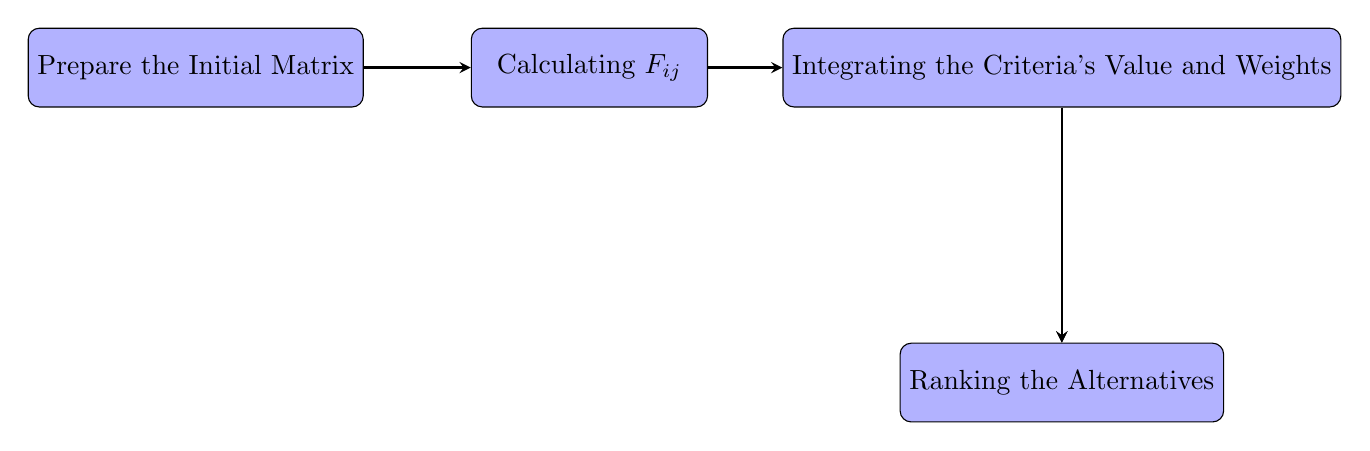
\begin{tikzpicture}[node distance=3cm]

% Nodes
\node (start) [block] {Prepare the Initial Matrix};
\node (process1) [block, right of=start, xshift=2cm] {Calculating $F_{ij}$};
\node (process2) [block, right of=process1, xshift=3cm] {Integrating the Criteria's Value and Weights};
\node (end) [block, below of=process2, yshift=-1cm] {Ranking the Alternatives};

% Arrows
\draw [arrow] (start) -- (process1);
\draw [arrow] (process1) -- (process2);
\draw [arrow] (process2) -- (end);

% Additional arrow downward from process2
%\node (decision1) [decision, below of=process1, yshift=-3cm] {};
\draw [arrow] (process2.south) -- ++(0,-1) -- (end);

\end{tikzpicture}
\end{center}

\textbf{Step 1:}This is an optional step that helps to conduct the following steps better.\\

The initial matrix is prepared based on the values for m$*$n matrix $r_{ij}$ is the value of the $i^{th}$ criterion for $j^{th}$ object where :

\begin{itemize}
    \item i = 1,2,...,m;
    \item j = 1,2,...,n;
\end{itemize}

Another point is to determine the weights of the
criteria ($w_{i}$) to show their importance. These weights
can be considered as numbers between zero and one
(or by percentages) and considering $\sum\limits^{n}_{i=1}w_{i}=1$\\

\textbf{Step 2:} Normalizing the Value of $i^{th}$ Criterion
for the $j^{th}$ Alternative (Calculating $\overline{r_{ij}}$):\\

The $\overline{r_{ij}}$ is known as the normalized $i^{th}$ criterion’s value for $j^{th}$ alternative/object. This value must be calculated in this step considering whether the problem is a cost or benefit type. The difference is that
in the cost problems the object is minimizing, on the other hand maximizing is the object of a benefit problem. These differences reflect in the $\overline{r_{ij}}$ calculation as follows:\\
\begin{eqnarray*}
\overline{r_{ij}}&=&\frac{\min (r_{ij})}{r_{ij}} ; \text{if j is a cost attribute.}\\
\overline{r_{ij}}&=&\frac{r_{ij}}{\max(r_{ij})} ; \text{if j is a benefit/profit attribute.}
\end{eqnarray*}

where $r_{ij}$ is the value of the $i^{th}$ criterion for $j^{th}$ object. The $min (r_{ij})$ is the largest value of the $i^{th}$ criterion when all alternatives are compared, and in contrast, $min (r_{ij})$ is the smallest value for it. Therefore,
 $\overline{r_{ij}}$ is a normalized value for the $i^{th}$ criterion and $j^{th}$
alternative.\\

\textbf{Step 3:} Integrating the Values of the Criteria and
Weights.\\

The integration of the criteria and weights helps
to gain a single magnitude that is the final performance value for each alternative. For this, the following equation can be used for the $j^{th}$ alternative/
object:\\
\begin{center}
    $S_{j}=\sum\limits^{n}_{n=1}w_{i}\overline{r_{ij}}$
\end{center}

\textbf{Step 4:} Ranking the Alternatives to Choose the
best One.\\

In the final step, the best alternative is chosen based on the largest performance value of the $S_{j}$ maximizing criterion, and the smallest for the minimizing criterion. Numerical examples are provided in the literature.\\

Finally, there is another important consideration for the SAW method that is beneficial to be noted
here:\\

The $r_{ij}$ is this method should be positive. According to this requirement the negative values should be transferred to positive ones $(\overline r_{ij})$ using different methods. For example, the following formula can be used:
\begin{center}

   $\overline r_{ij} = r_{ij} + |{min (r_{ij})}|+1$
    
\end{center}

\subsection{APPLICATION AREA, MERITS, AND DEMERITS OF THE SAW}
\hspace{1em}The SAW method possesses different application
areas ranging from business to water management and financial studies. Different studies are conducted based on utilizing the SAW method for ranking and selection purposes [8]. This method can be also integrated with other MADM methods such as AHP, VIKOR, TOPSIS, and ELECTRE; some examples are as follows:
\begin{itemize}
    \item Ranking the cloud render farm services;

    \item Evaluating the quality of urban life;

    \item Risk assessment in public-private partnership projects;

    \item Selecting the most efficient devices;

    \item Selecting sensors attached to the devices;

    \item Ranking the best resources at the local or lower level;


\end{itemize}

Figure 1  is based on the SAW search term in the “ScienceDirect” database (conducted on 2022/06/2). The figure illustrates that according to the results this method is mostly used in the engineering, computer, environmental, and decision sciences subject areas.

\begin{figure}
    \centering
    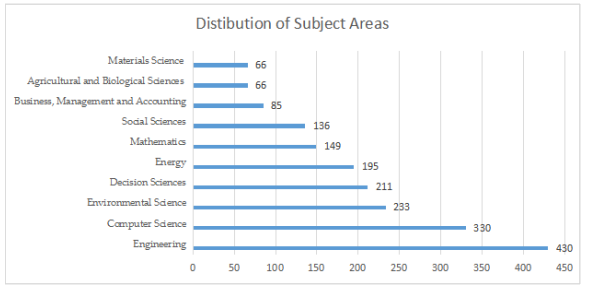
\includegraphics[width=0.7\linewidth]{tab.png}
    \caption{Distribution of subject areas used the SAW method.}

\end{figure}

\subsection{THE BASICS OF THE TOPSIS METHOD AND PROBLEMS OF ITS FUZZY EXTENSION}

\hspace{1em}The classical TOPSIS method is based on the idea that the best alternative should have the shortest distance from the positive ideal solution and the greatest distance from the negative one. It is assumed that if each local criterion is monotonically increasing or decreasing, then it is easy to define the ideal solution [18].\\

A positive ideal solution is composed of all the best achievable values of the local criteria, while a negative ideal solution is compose d of all the worst achievable values of the local criteria.\\

Suppose a MCDM problem is based on m alternatives $A_{1}, A_{2}, ... , A_{m}$ and n local criteria $C_{1},C_{2}, ... , C_{n}$. Each alternative is evaluated with respect to the n criteria. All the ratings are assigned to alternatives and presented in the decision matrix $D[x_{ij}]_{m*n}$, where $x_{ij}$ is the rating of alternative $A_{i}$ with respect to the criterion $C_{j}$. Let $W = [w_{1}, w_{2}, ... , w_{n}]$ be the vector of local criteria weights satisfying $\sum\limits^{n}_{j=1}w_{j}=1$\\
The TOPSIS method consists of the following steps :

\begin{enumerate}
    \item \textbf{Normalize the decision matrix:}
    \begin{center}

    $r_{ij}=\frac{x_{ij}}{\sqrt{\sum\limits^{m}_{k=1}x^{2}_{kj}}}$,i=1,2,...,m;  j=1,2,...,n;
    
    \end{center}
Multiply the columns of normalized decision matrix by the associated weights:

\begin{center}

$v_{ij} = w_{i} * r_{ij}$,i=1,2,...,m;  j=1,2,...,n;

\end{center}

\item \textbf{Determine the positive ideal and negative ideal solutions, respectively, as follows:}
\begin{center}
    $A^{+} = \{v^{+}_{1}, v^{+}_{2},...,v^{+}_{n}\} = \{(maxv_{ij}|j\in K_{b}) (minv_{ij}|j \in k_{c})\} $\\

    $A^{-} = \{v^{-}_{1}, v^{-}_{2},...,v^{-}_{n}\} = \{(minv_{ij}|j\in K_{b}) (maxv_{ij}|j \in k_{c})\} $

    
\end{center}

where $K_{b}$ is a set of benefit criteria and $K_{c}$ is a set of cost criteria

\item \textbf{Obtain the distances of the existing alternatives from the positive ideal and negative ideal solutions:} two Euclidean distances for each alternatives are, respectively, calculated as follows:
\begin{center}

$S_{i}^{+}=\sqrt{\sum\limits_{j=1}^{n}(v_{ij}-v_{j}^{+}})^{2}$, i= 1,2,...,m\\
   $S_{i}^{-}=\sqrt{\sum\limits_{j=1}^{n}(v_{ij}-v_{j}^{-}})^{2}$, i= 1,2,...,m 
\end{center}

\item \textbf{Calculate the relative closeness to the ideal alternatives:} 
\begin{center}

$RC_{i}=\frac{S_{i}^{-}}{S_{i}^{+}+S^{-}_{i}}$ ;i= 1, 2, ... , m; $0\leq RC_{i}\leq 1$    
\end{center}

\item \textbf{Rank the alternatives according to their relative closeness to the ideal alternatives:} The bigger $RC_{i}$, the better alternative $A_{i}$. Let us consider a formal fuzzy extension of the classical TOPSIS method in a form which is free of the simplifications and limitations associated with the known fuzzy TOPSIS methods analyzed in the previous section.[1] It is important that such an approach makes it possible to present the fuzzy TOPSIS method in the form of a weighted sum aggregation of the local criteria. Suppose a MCDM problem is based on m alternatives $A_{1}, A_{2}, ... , A_{m} $and n criteria $C_{1}, C_{2}, ... , C_{n}$. Let $D[\overline{x_{ij}}]_{m*n}$ be a fuzzy decision matrix, where $\overline{x_{ij}}=(a_{ij},b_{ij},c_{ij})$ is a triangular fuzzy value representing the rating of alternative $A_{i}$ with respect
to the criterion $C_{j}$. Let $W = [w_{1},w_{2}, ... , w_{n}]$ be the vector of real-valued local criteria weights satisfying $\sum\limits^{n}_{j=1}w_{j}=1$\\

The method of formal fuzzy extension of TOPSIS method consists of the following steps:
\begin{enumerate}
    \item Normalizing the decision matrix.\\
An appropriate and methodologically justified method for normalization of fuzzy decision matrices was developed in as follows:
\begin{center}
$\overline{r_{ij}}=(r_{ij}^{L},r_{ij}^{M},r_{ij}^{U})=(\frac{a_{ij}}{c_{j}^{+}},\frac{b_{ij}}{c_{j}^{+}},\frac{c_{ij}}{c_{j}^{+}})$;i=1,...,m;$j \in K_{b}$,
    
\end{center}

where $c^{+}_{j}=max_{i}(c_{ij});j \in K_{b}$.

\begin{center}

$\overline{r_{ij}}=(r_{ij}^{L},r_{ij}^{M},r_{ij}^{U})=(\frac{a_{ij}}{c_{j}^{-}},\frac{b_{ij}}{c_{j}^{-}},\frac{c_{ij}}{c_{j}^{-}})$;i=1,...,m;$j \in K_{c}$,
    
\end{center}
where $a^{+}_{j}=min_{i}(a_{ij});j \in K_{c}$.
This normalization guarantees that $\overline{r_{ij}}\subset [0,1]$ for all i and j.


\item The positive and negative ideal solutions are obtained as follows:

\begin{center}

$A_{+}=\{\overline{r^{+}_{1}},\overline{r^{+}_{2}},...,\overline{r^{+}_{n}}\}=\{max\{(r_{ij}^{L},r_{ij}^{M},r_{ij}^{U})\}|j\in K_{b}, min\{(r_{ij}^{L},r_{ij}^{M},r_{ij}^{U})\}|j\in K_{c}\},$


$A_{-}=\{\overline{r^{-}_{1}},\overline{r^{-}_{2}},...,\overline{r^{-}_{n}}\}=\{min\{(r_{ij}^{L},r_{ij}^{M},r_{ij}^{U})\}|j\in K_{b}, max\{(r_{ij}^{L},r_{ij}^{M},r_{ij}^{U})\}|j\in K_{c}\},$
  
\end{center}
\item Calculation of separation of each alternative from the positive and negative ideal solutions.

\begin{center}

$\overline{r_{j}^{+}} \geq \overline{r_{ij}} , i=1,2...m , j \in K_{b}$

$\overline{r_{ij}} \geq \overline{r_{j}^{+}} , i=1,2...m , j \in K_{c}$

$\overline{r_{ij}} \geq \overline{r_{j}^{-}} , i=1,2...m , j \in K_{b}$

$\overline{r_{j}^{-}} \geq \overline{r_{ij}} , i=1,2...m , j \in K_{c}$
    
\end{center}

Therefore, there is no need to use n-dimensional Euclidean or Hamming distances for obtaining $S_{i}^{+}$and $S_{i}^{-}$ i = 1, 2,..., m, as they can be calculated as follows:

\begin{center}  

$S_{i}^{+}=\sum\limits_{j \in K_{b}}w_{j}(\overline{r_{j}^{+}}-\overline{r_{ij}})+\sum\limits_{j \in K_{c}}w_{j}(\overline{r_{ij}}-\overline{r_{j}^{+}})$

$S_{i}^{-}=\sum\limits_{j \in K_{b}}w_{j}(\overline{r_{ij}}-\overline{r_{j}^{-}})+\sum\limits_{j \in K_{c}}w_{j}(\overline{r_{j}^{-}}-\overline{r_{ij}})$

\end{center}

These expressions make it possible to look at the problem from another point of view. We can see that the expressions 

\begin{center}

$\overline{r_{j}^{+}} - \overline{r_{ij}} , i=1,2...m , j \in K_{b}$

$\overline{r_{ij}} - \overline{r_{j}^{+}} , i=1,2...m , j \in K_{c}$

$\overline{r_{ij}} - \overline{r_{j}^{-}} , i=1,2...m , j \in K_{b}$

$\overline{r_{j}^{-}} - \overline{r_{ij}} , i=1,2...m , j \in K_{c}$
    
\end{center}

may be treated as modified values of local criteria based on the initial ones. Therefore, expressions may be considered as the weighted sum aggregation s of local criteria. Nevertheless, this aggregation cannot be treated as unique nor as the best one within the framework of the fuzzy TOPSIS method in all case 
\end{enumerate}

\end{enumerate}

An important property of weighted sum aggregation is that the small values of some local criteria may be counterbalanced by large values of other ones in the final assessment. For example, a high percent of goods of low quality in most cases cannot be counterbalanced by low production costs, just as the low professional qualifications of medical staff usually cannot be compensated for by high quality diagnostic equipment and so on. Since this compensation property of weighted sum aggregation is in many applications undesirable, a decision maker may prefer to use, e.g., weighted geometric aggregation and a more cautious decision maker may prefer aggregation based on the ‘‘principle of maximal pessimism’’. \\

The problem of selecting an appropriate aggregation method is of perennial interest, because of its direct relevance to practical decision making.[4] Generally, the choice of aggregation mode is a context dependent problem. Therefore, in different applications of the TOPSIS method, different aggregation modes may be used to obtain $S^{+}$ and $S^{-}$. Of course, currently the most popular aggregating mode is the weighted sum. It is used in many well known decision making models, but often without any critical analysis. On the other hand, in some fields, e.g., in ecological modelling, the weighted sum is not used for aggregation. The reason behind this is that in practice there are cases when if any local criterion is totally dissatisfied then the considered alternative should be rejected from the consideration completely. Nevertheless, when dealing with a complex task characterized by a great number of local criteria, it seems reasonable to use all those types of aggregation relevant to this task. If the results obtained by using different aggregation modes are similar, this fact may be considered as good confirmation of their optimality.\\

In the opposite case, additional analysis of local criteria and their ranking is usually advised. In addition to the weighted sum, we propose to use other types of aggregations in the fuzzy TOPSIS method. Since different aggregation modes may provide different final rankings of alternatives, to obtain a compromise result, we propose a new method for generalizing the aggregation modes within the framework of the fuzzy TOPSIS method. This method is based on an adaptation of the approach developed, which is based on the synthesis of Type 2 and Level 2 fuzzy sets To calculate the fuzzy values we shall use the a-cut representation of fuzzy values. This means that there are no restrictions on the form of the fuzzy values in our approach and we use triangular fuzzy values in the above definitions only to make the presentation of the developed approach more transferable. Of course, when the fuzzy values have regular triangular or trapezoidal forms, the solution to a MCDM problem with the use of the TOPSIS method can be reduced in its consideration to only the lowest and highest $\alpha$-cuts, practically without any loss of accuracy.


\subsection{APPLICATION AREA, MERITS AND DEMERITS OF THE 
FUZZY TOPSIS}

\subsubsection*{APPLICATION AREA [13]:}
\begin{enumerate}
    \item \textbf{Healthcare:} Evaluating treatment options, hospital performance, and patient care services, considering multiple criteria such as cost, efficacy, and patient satisfaction.

    \item \textbf{Supply Chain Management:} Selecting suppliers based on criteria like quality, delivery time, and cost, accommodating the uncertainty in supplier performance.


    \item \textbf{Environmental Management:} Assessing environmental impact, sustainability practices, and resource allocation, where data can be uncertain or imprecise.


    \item \textbf{Finance: Portfolio} selection, investment analysis, and risk assessment, integrating various economic indicators and qualitative judgments.


    \item \textbf{Manufacturing:} Evaluating production processes, machinery selection, and quality control by considering multiple conflicting criteria.


    \item \textbf{Manufacturing:} Evaluating production processes, machinery selection, and quality control by considering multiple conflicting criteria.

\end{enumerate}

\subsubsection*{MERITS:}
\begin{enumerate}
    \item \textbf{Handling Uncertainty:} Fuzzy TOPSIS effectively manages uncertainty and imprecision in decision-making by allowing for degrees of membership rather than binary outcomes.


    \item \textbf{Comprehensive Evaluation:} It enables the integration of both qualitative and quantitative criteria, providing a holistic view of the alternatives.


    \item \textbf{Ranking Alternatives:} The method facilitates a clear ranking of options, making it easier for decision-makers to identify the best choice.


    \item \textbf{Flexibility:} It can be adapted to various domains and decision-making scenarios, making it versatile for different applications.


    \item \textbf{User-Friendly:} The approach is intuitive and can be implemented with relative ease, allowing decision-makers from non-technical backgrounds to use it effectively.

\end{enumerate}

\subsubsection*{DEMERITS:}
\begin{enumerate}
    \item \textbf{Complexity in Data Collection:} Gathering fuzzy data and defining membership functions can be challenging and may require expert input, which can be subjective.


    \item \textbf{Parameter Sensitivity:} The results can be sensitive to the chosen membership functions and the weight assigned to different criteria, potentially leading to biased outcomes.


    \item \textbf{Computationally Intensive:} For large datasets or complex problems, the computational load may become significant, requiring advanced software or longer processing times.


    \item \textbf{Lack of Standardization:} There is no universally accepted methodology for defining fuzzy sets and membership functions, which can lead to inconsistencies in application.


    \item \textbf{Interpretation Challenges:} The results may be difficult to interpret for stakeholders unfamiliar with fuzzy logic concepts, potentially complicating the decision-making process.
\end{enumerate}



\newpage
\begin{center}
    \section*{CHAPTER – IV}
\end{center}
\section{APPLICATION}
The TOPSIS method involves the following key techniques:
\begin{enumerate}
    \item \textbf{Normalization }of data to bring it to a comparable scale.
    \item \textbf{Weighting} of normalized data to reflect the importance of each criterion.
    \item \textbf{Identification} of ideal and negative-ideal solutions for comparison.
    \item \textbf{Calculation} of distances from the ideal and negative-ideal solutions.
    \item \textbf{Computation} of the closeness coefficient to rank alternatives.
\end{enumerate}

These steps help in evaluating and selecting alternatives that are closest to the ideal solution while being farthest from the negative-ideal solution, thus facilitating informed decision-making [22]. The paper also included a dataset on diabetes in which the scale point was fixed using linguistic values some beneficial and non-beneficial attributes are mentioned according to the weightage. The ranking result was eventually discovered, and visualization was displayed using the MATLAB programming language. The major contribution of this paper as follows, 
\begin{itemize}
    \item Using the average approach, the acquired dataset is categorized by age wise.
    \item For the impacted diabetes patient’s dataset, linguistic values are provided. 
    \item The scale point is fixed based on linguistic values, and the weighting of beneficial and non-beneficial value is fixed based on the dataset. 
    \item With the use of the TOPSIS approach, the dataset's final ranking is established. 
    \item Using MATLAB the visualization result is determined. 
\end{itemize}
There are five steps of algorithms to solve our problem\\
\textbf{Step 1:} Data collection\\
\textbf{Step 2:} Data categorize to simplify the dataset \\
\textbf{Step 3:} Fixing scale point with respect to linguistic values\\
\textbf{Step 4:} Fixing the weightage, beneficial and non-beneficial of the simplified dataset \\
\textbf{Step 5:} Find ranking using Multi Criteria decision method of TOPSIS method.

\begin{figure}
\subsection{DATASET WITH OUTCOME}
    \centering
    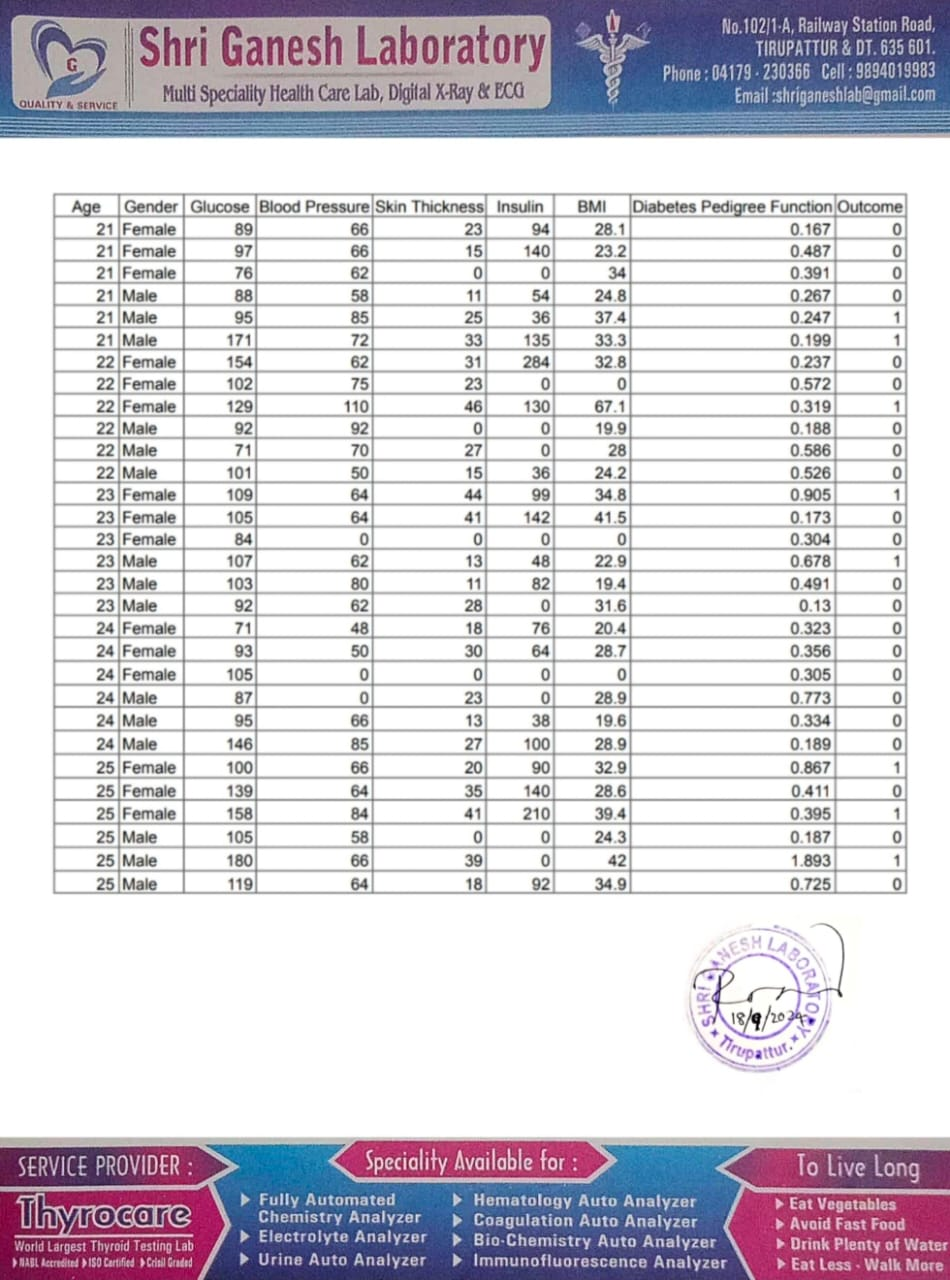
\includegraphics[width=1\linewidth]{lab_1.jpg}
    \caption{ }
    \label{fig:2}
\end{figure}


\begin{figure}
    \centering
    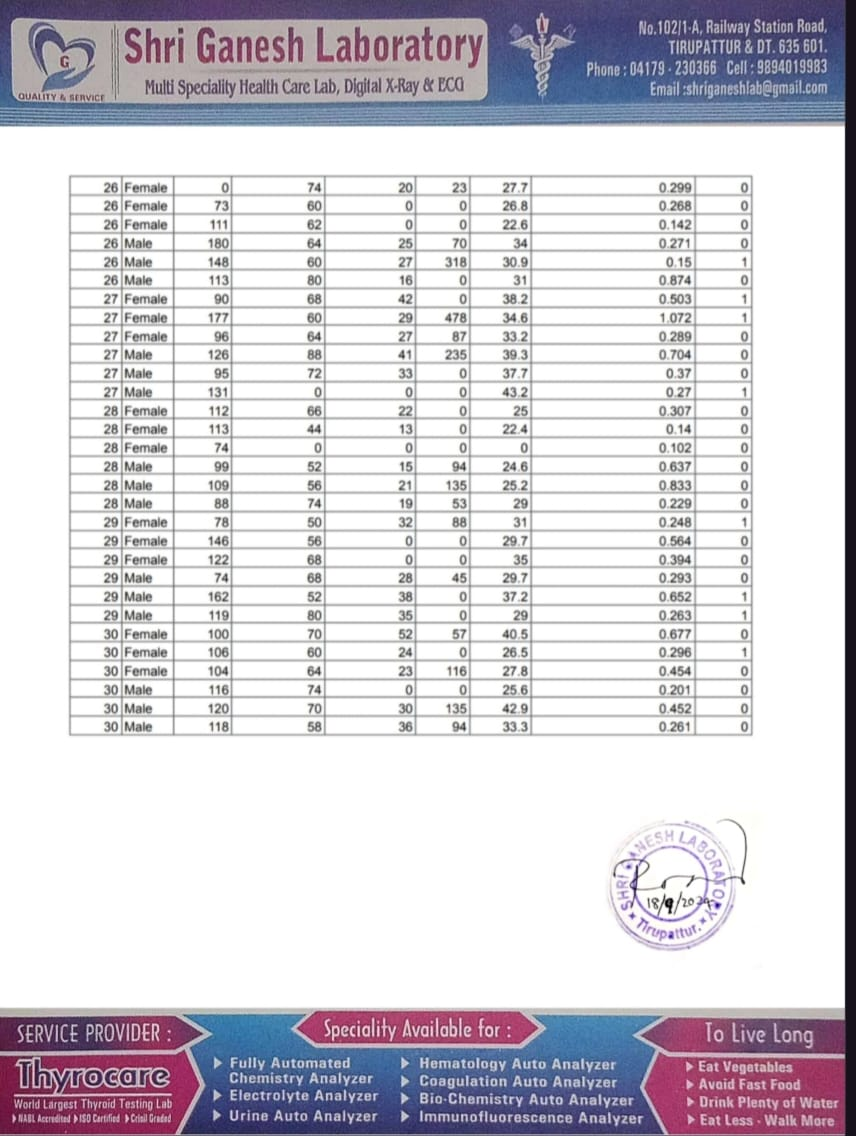
\includegraphics[width=1\linewidth]{lab_2.jpg}
    \caption{}
    \label{fig:enter-label}
\end{figure}

\begin{figure}
    \centering
    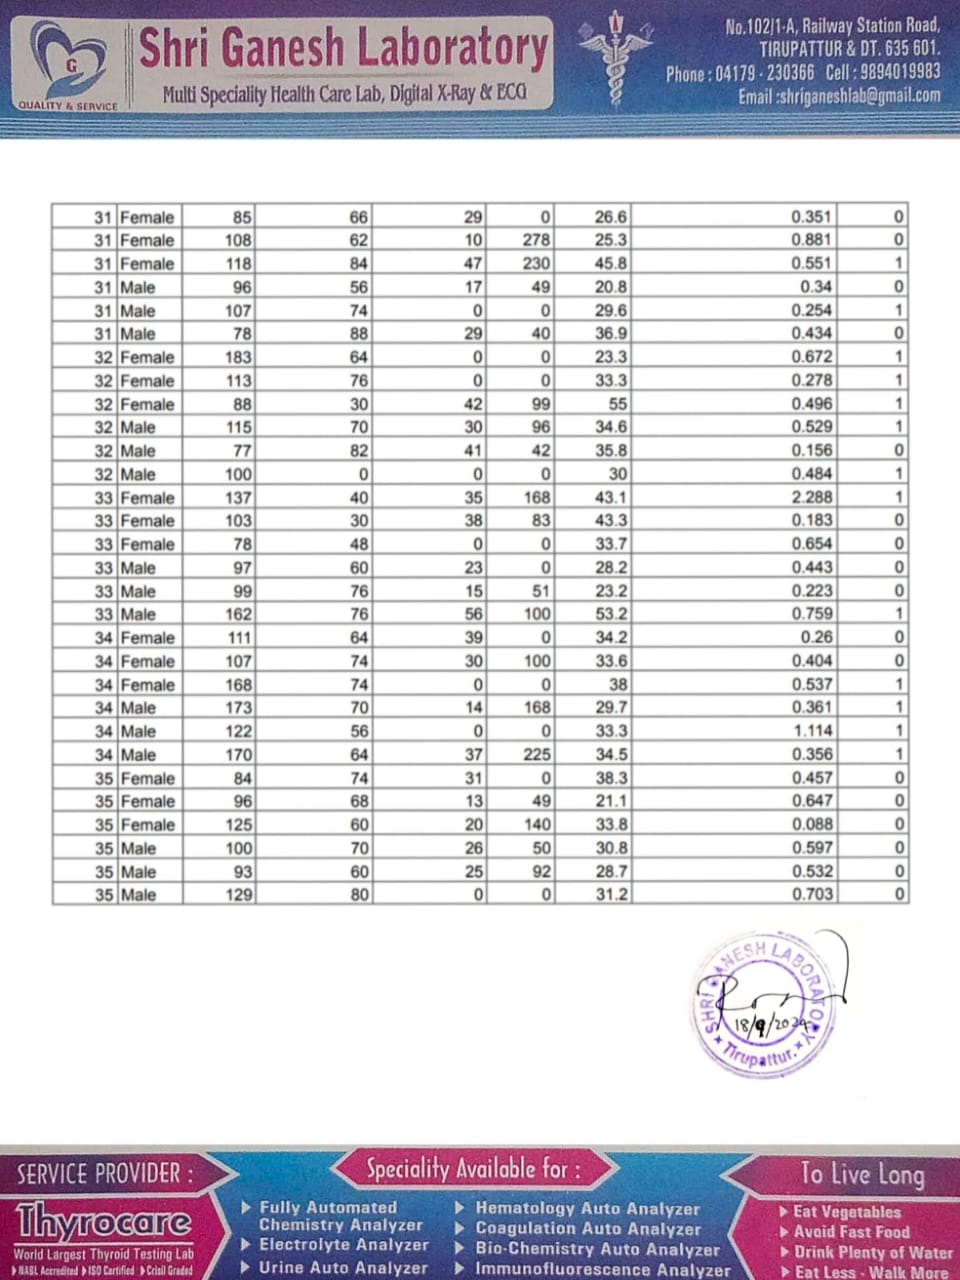
\includegraphics[width=1\linewidth]{lab_3.jpg}
    \caption{}
    \label{fig:enter-label}
\end{figure}

\begin{figure}
    \centering
    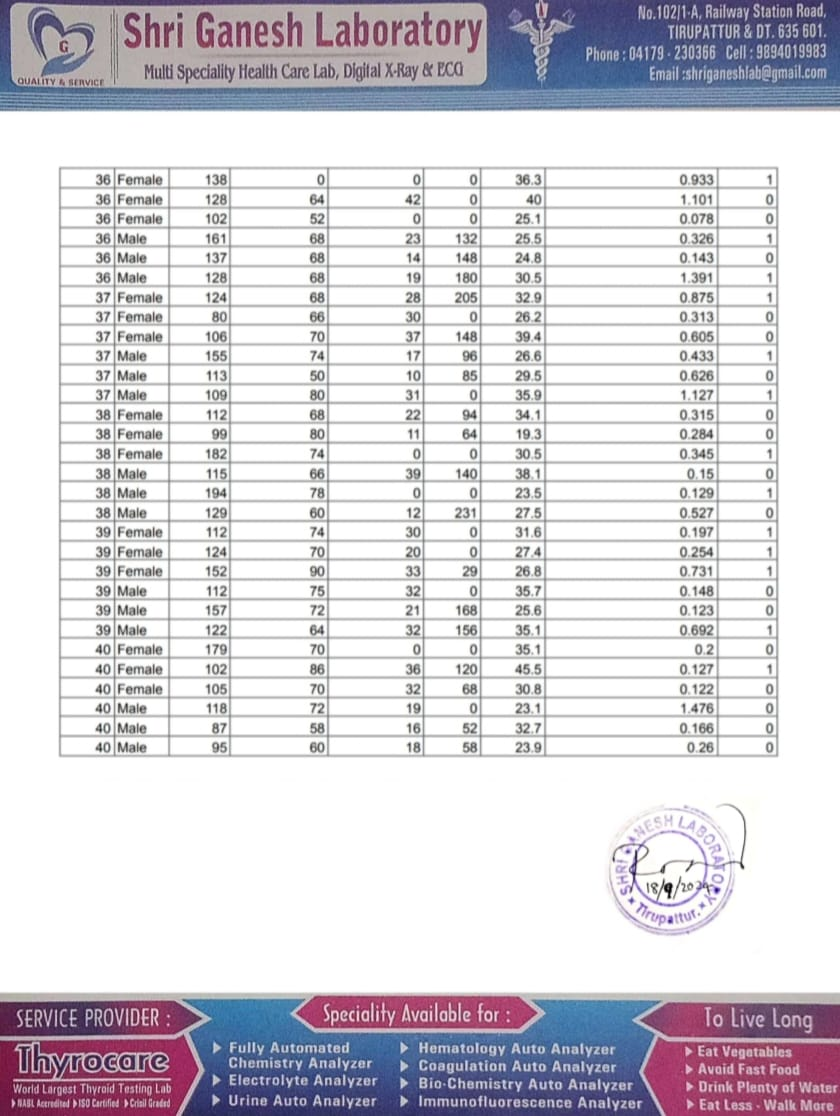
\includegraphics[width=1\linewidth]{lab_4.jpg}
    \caption{}
    \label{fig:enter-label}
\end{figure}

\begin{figure}
    \centering
    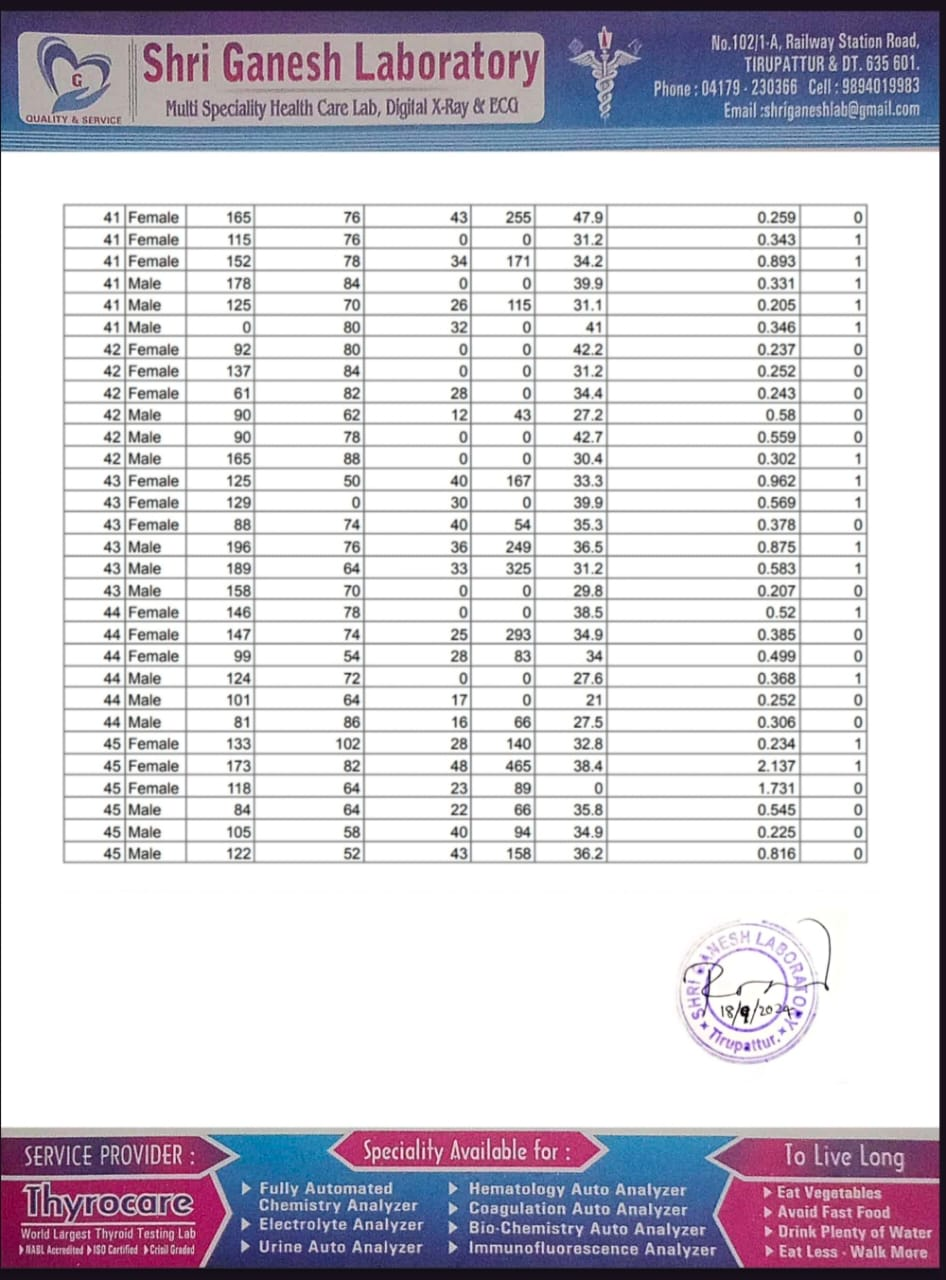
\includegraphics[width=1\linewidth]{lab_5.jpg}
    \caption{}
    \label{fig:enter-label}
\end{figure}

\begin{figure}
    \centering
    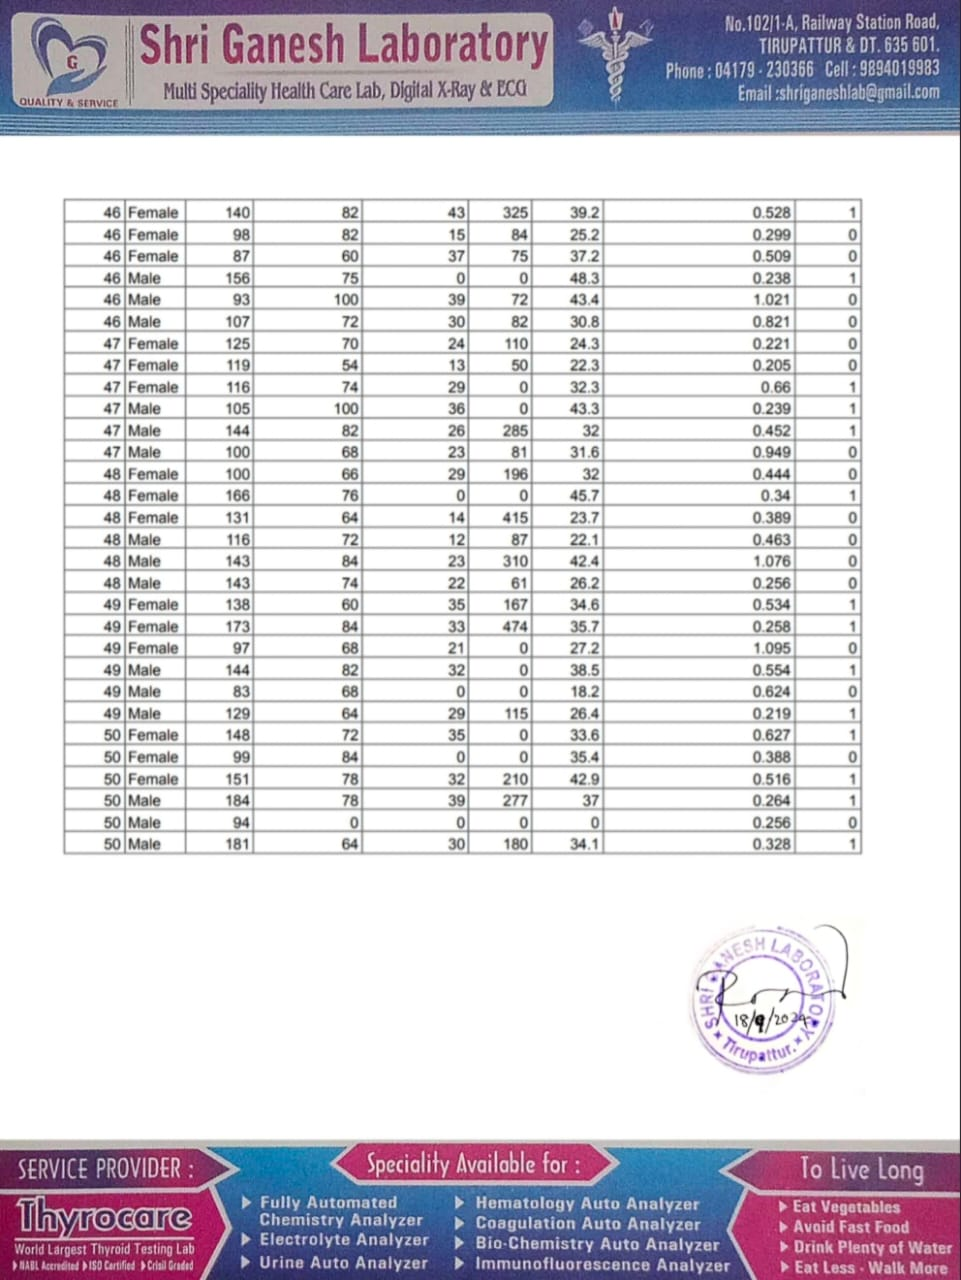
\includegraphics[width=1\linewidth]{lab_6.jpg}
    \caption{}
    \label{fig:enter-label}
\end{figure}

\begin{figure}
    \centering
    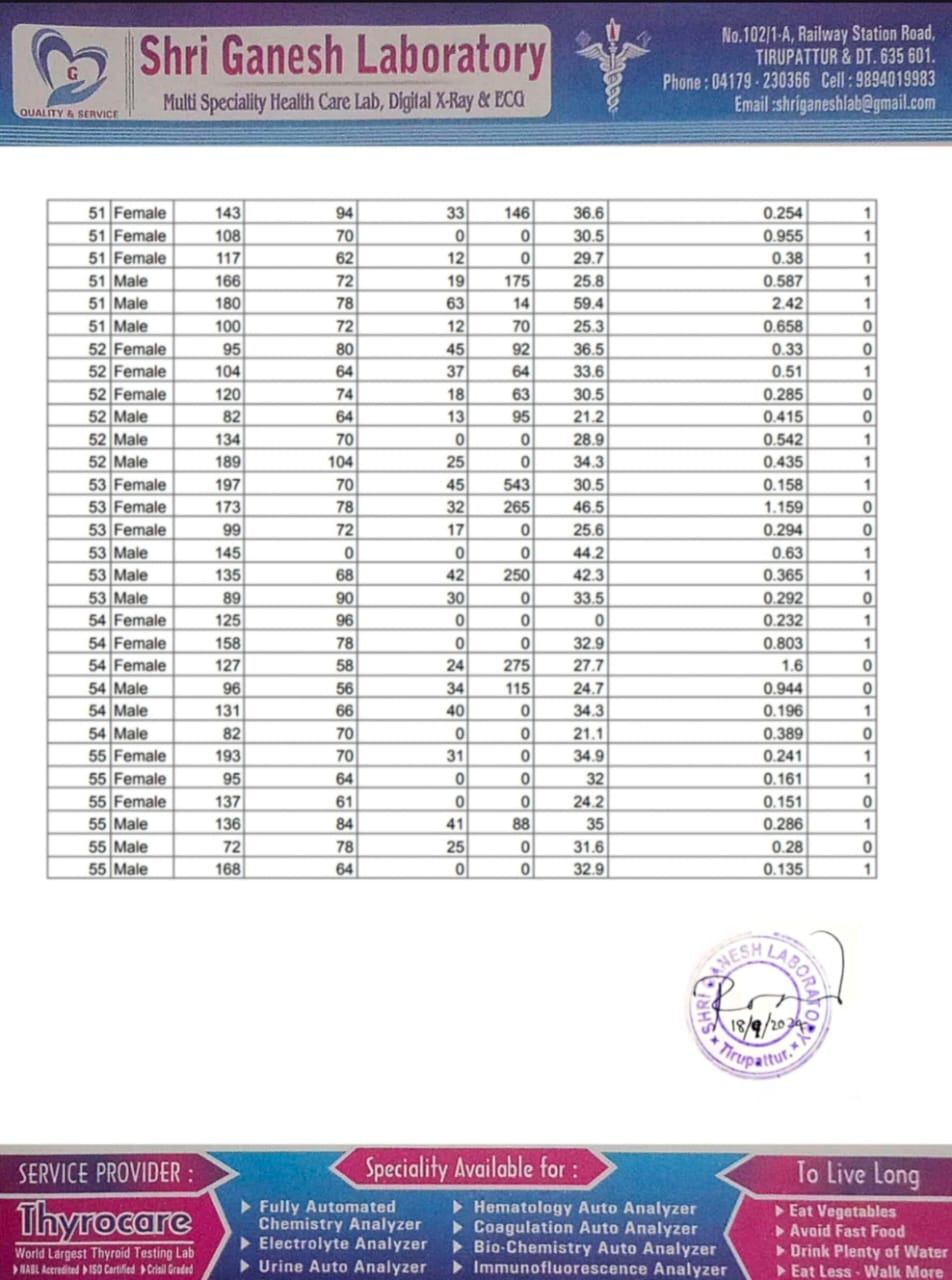
\includegraphics[width=1\linewidth]{lab_7.jpg}
    \caption{}
    \label{fig:enter-label}
\end{figure}

\begin{figure}
    \centering
    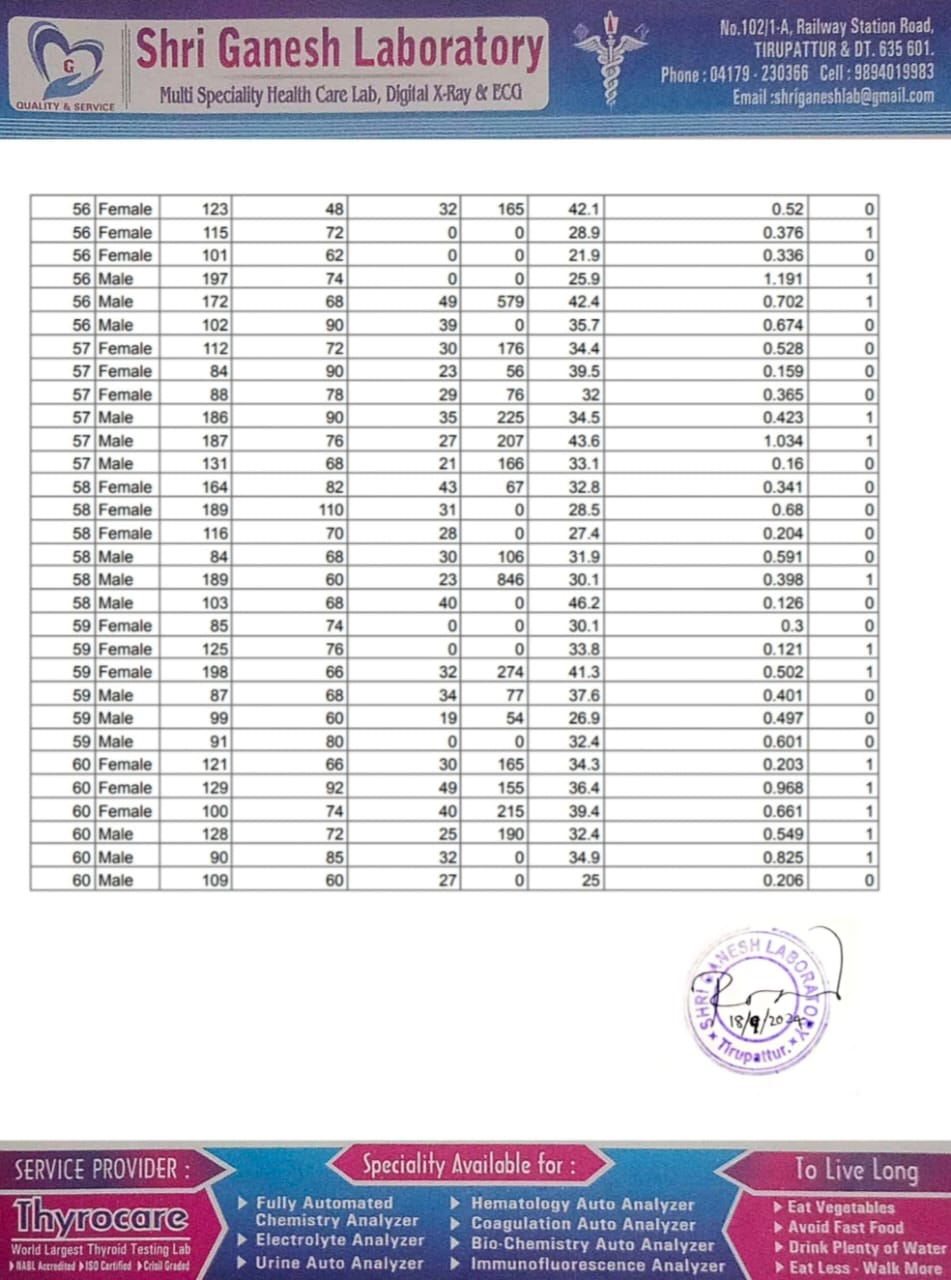
\includegraphics[width=1\linewidth]{lab_8.jpg}
    \caption{}
    \label{fig:enter-label}
\end{figure}

\begin{figure}
    \centering
    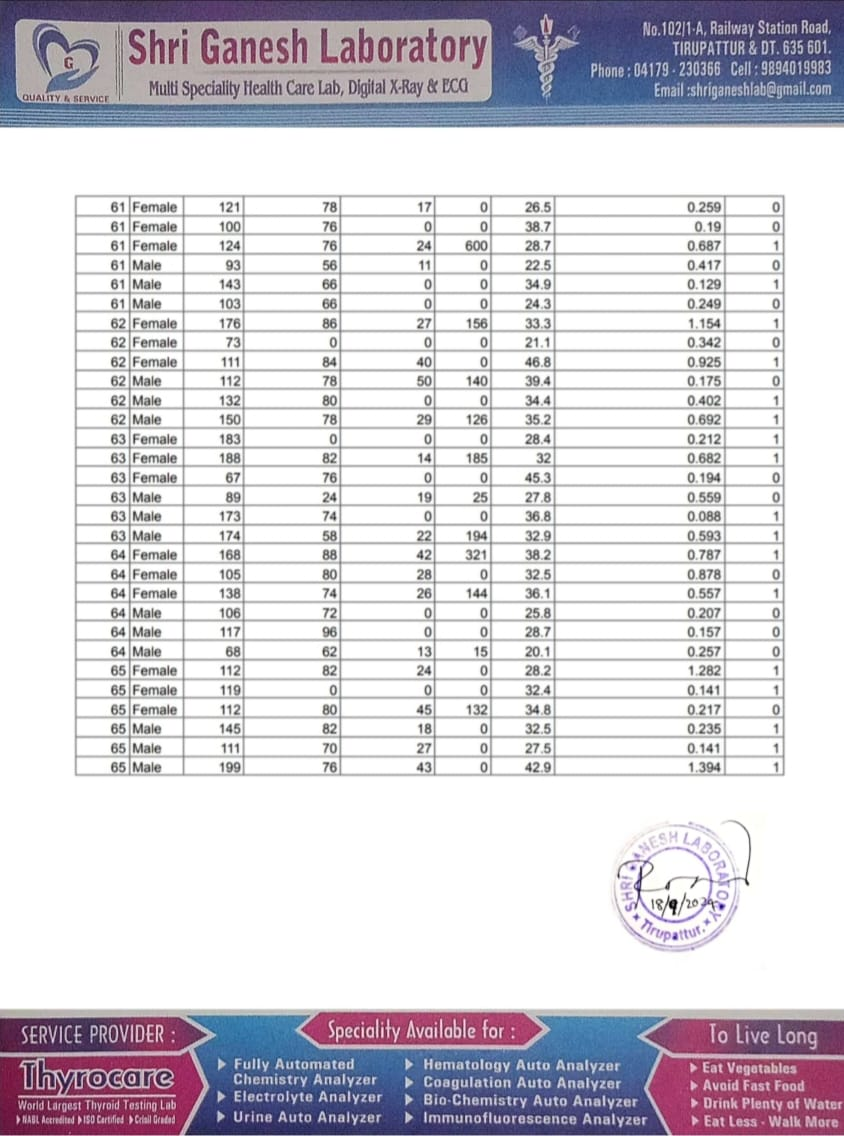
\includegraphics[width=1\linewidth]{lab_9.jpg}
    \caption{}
    \label{fig:enter-label}
\end{figure}

\begin{figure}
    \centering
    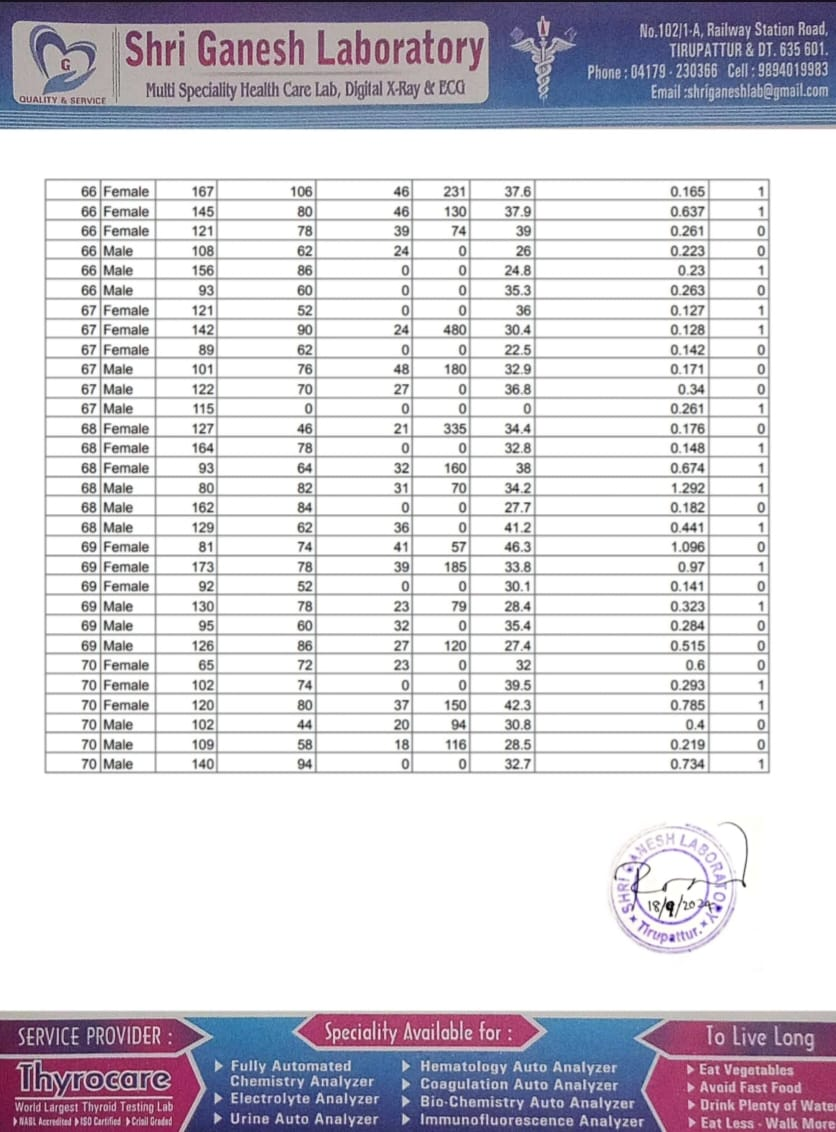
\includegraphics[width=1\linewidth]{lab_10.jpg}
    \caption{}
    \label{fig:enter-label}
\end{figure}

\subsection{IMPLEMENTATION OF SAW}


\textbf{Step 1:} Categorize Dataset
\begin{itemize}
\item \textbf{Case 1:} The Dataset mentioned above[4.3] was obtained from the “ShriGanesh Laboratory, Tirupattur District.”
\item \textbf{Case 2:} The dataset from case 1, which contains the records of 300 people (150 males and 150 females), was gathered to determine which age group of people will be most susceptible to the emerging viral threats.
\end{itemize}
\textbf{Step 2:}The dataset was categorized by determining the average for each age group, as shown
in table 1.\\

\begin{table}[h]
\centering
 \resizebox{\textwidth}{!}{
\begin{tabular}{|c|c|c|c|c|c|c|}
\hline
\textbf{Age} & \textbf{Glucose} & \textbf{Blood Pressure} & \textbf{Skin Thickness} & \textbf{Insulin} & \textbf{BMI} & \textbf{Diabetes Pedigree Function} \\
\hline
21-25  & 108.7667  & 61.7         & 21.66667     & 69.66666667 & 27.72    & 0.454167   \\
26-30  & 110       & 60.4666667   & 21.6         & 67.6        & 30.45333 & 0.407167   \\
31-35  & 114.0667  & 63.2         & 21.56666667  & 68.66666667 & 33.63    & 0.5344     \\
36-40  & 125.9     & 67.16666667  & 20.8         & 72.46666667 & 30.63333 & 0.473233333\\
41-45  & 122.93333 & 70.73333333  & 21.46666667  & 94.43333333 & 33.36667 & 0.538066667\\
46-50  & 127       & 71.9         & 23.36666667  & 121.8666667 & 32.18667 & 0.492433333\\
51-55  & 129.8667  & 70.9         & 21.26666667  & 75.16666667 & 31.54    & 0.536233333\\
56-60  & 126.8333  & 73.96666667  & 25.6         & 126.6333333 & 33.84667 & 0.488066667\\
61-65  & 127.06667 & 66.66666667  & 17.3         & 67.93333333 & 32.29    & 0.4734     \\
65-70  & 119       & 69.6         & 21.13333333  & 82.03333333 & 32.49    & 0.407366667\\
\hline
\end{tabular}
}
\caption{Health Data by Age Group}
\end{table}
\textbf{Step 3:} Fixing the weightage as 0.166 and multiplying it with the table 1, we the following table 2.

\begin{table}[h]
\centering
\resizebox{\textwidth}{!}{
\begin{tabular}{|c|c|c|c|c|c|c|}
\hline
\textbf{Age} & \textbf{Glucose} & \textbf{Blood Pressure} & \textbf{Skin Thickness} & \textbf{Insulin} & \textbf{BMI} & \textbf{Diabetes Pedigree Function} \\
\hline
21-25  & 18.0552722  & 10.2422      & 3.59666722   & 11.56466667 & 4.60152    & 0.075391722   \\
26-30  & 18.26       & 10.03746672  & 3.5856       & 11.2216     & 5.055253333 & 0.067589722   \\
31-35  & 18.9350722  & 10.4912      & 3.580066667  & 11.39866667 & 5.58258    & 0.0887104     \\
36-40  & 20.8994     & 11.14966667  & 3.4528       & 12.02946667 & 5.0853278  & 0.078556733   \\
41-45  & 20.4069328  & 11.74173333  & 3.563466667  & 15.67593333 & 5.53866722 & 0.089319067   \\
46-50  & 21.082      & 11.9354      & 3.878866667  & 20.22986667 & 5.3429872  & 0.081749333   \\
51-55  & 21.5578672  & 11.7694      & 3.530266667  & 12.47766667 & 5.23564    & 0.089043133   \\
56-60  & 21.0543328  & 12.27846667  & 4.2496       & 21.02113333 & 5.6184752  & 0.081019067   \\
61-65  & 21.0930672  & 11.06666667  & 2.8718       & 11.27693333 & 5.36014    & 0.0785844     \\
66-70  & 19.754      & 11.5536      & 3.508133333  & 13.61753333 & 5.39343    & 0.067622867   \\
\hline
\end{tabular}
}
\caption{Average Weightage by Age Group}
\end{table}
\textbf{Step 4:} Ranking is given accruing to the result of total value, from minimum to maximum as shown in the table 3.

\newpage
\begin{table}[h]
\centering
\begin{tabular}{|c|c|c|}
\hline
\textbf{Age} & \textbf{Total} & \textbf{Ranking} \\
\hline
21-25  & 48.13571781  & 10 \\
26-30  & 48.22750978  & 9  \\
31-35  & 50.07629593  & 8  \\
36-40  & 52.69502285  & 6  \\
41-45  & 57.0162524   & 3  \\
46-50  & 62.55086449  & 2  \\
51-55  & 54.65985529  & 4  \\
56-60  & 64.30309906  & 1  \\
61-65  & 51.74719162  & 7  \\
66-70  & 53.89422953  & 5  \\
\hline
\end{tabular}
\caption{Total Score and Ranking by Age Group}
\end{table}

From the above ranking we get to know that the diabetic people between the age 56-60 are the most susceptible for the emerging viral threats.

\subsection{IMPLEMENTATION OF FUZZY TOPSIS}
\textbf{Step 1:} Categorize Dataset
\begin{itemize}
\item \textbf{Case 1:} The Dataset mentioned above [4.2] was obtained from the “ShriGanesh Laboratory, Tirupattur District.”
\item \textbf{Case 2:} The dataset from case 1, which contains the records of 300 people (150 males and 150 females), was gathered to determine which age group of people will be most susceptible to the emerging viral threats.
\end{itemize}
\textbf{Step 2:} The dataset was categorized by determining the average for each age group, as shown in table 4.

\begin{table}[h]
\centering
 \resizebox{\textwidth}{!}{
\begin{tabular}{|c|c|c|c|c|c|c|}
\hline
\textbf{Age} & \textbf{Glucose} & \textbf{Blood Pressure} & \textbf{Skin Thickness} & \textbf{Insulin} & \textbf{BMI} & \textbf{Diabetes Pedigree Function} \\
\hline
21-25  & 108.7667  & 61.7         & 21.66667     & 69.66666667 & 27.72    & 0.454167   \\
26-30  & 110       & 60.4666667   & 21.6         & 67.6        & 30.45333 & 0.407167   \\
31-35  & 114.0667  & 63.2         & 21.56666667  & 68.66666667 & 33.63    & 0.5344     \\
36-40  & 125.9     & 67.16666667  & 20.8         & 72.46666667 & 30.63333 & 0.473233333\\
41-45  & 122.93333 & 70.73333333  & 21.46666667  & 94.43333333 & 33.36667 & 0.538066667\\
46-50  & 127       & 71.9         & 23.36666667  & 121.8666667 & 32.18667 & 0.492433333\\
51-55  & 129.8667  & 70.9         & 21.26666667  & 75.16666667 & 31.54    & 0.536233333\\
56-60  & 126.8333  & 73.96666667  & 25.6         & 126.6333333 & 33.84667 & 0.488066667\\
61-65  & 127.06667 & 66.66666667  & 17.3         & 67.93333333 & 32.29    & 0.4734     \\
65-70  & 119       & 69.6         & 21.13333333  & 82.03333333 & 32.49    & 0.407366667\\
\hline
\end{tabular}
}
\caption{Health Data by Age Group}
\end{table}

\textbf{Step 3:} Choosing Scale Point

\begin{itemize}

\item \textbf{Case 1:} By consider the column of affected diabetes (Outcome), the possibility of
diabetes where fixed with the linguistic of the range [0,1]
\newpage
\begin{table}[h]
\centering
\begin{tabular}{|c|c|}
\hline
\textbf{RANGE} & \textbf{REMARK} \\
\hline
$0 \leq \text{POD}$  & \textbf{Very Low}  \\
\hline
$0.35 \leq \text{POD} \leq 0.44$  &  \textbf{Low} \\
\hline
$0.45 \leq \text{POD} \leq 0.49$ &  \textbf{Normal} \\
\hline
 $0.50 \leq \text{POD} \leq 0.59$ &  \textbf{High} \\
\hline
$0.6 \leq \text{POD}$ &  \textbf{Very High} \\
\hline
\end{tabular}
\caption{Linguistic Value for the Possibility of Diabetes}
\end{table}
\item \textbf{Case 2:} Table 6 displays the linguistic values for the Affected Diabetes Patient as determined in step 1
\begin{table}[h!]
\centering
\begin{tabular}{|c|c|c|}
\hline
\textbf{AGE} & \textbf{AFFECTED BY DIABETES} & \textbf{LINGUISTIC VALUE OF POD} \\
\hline
21-25 & 0.687875 & Very High \\
\hline
26-30 & 0.43175 & Low \\
\hline
31-35 & 0.667615 & Very High \\
\hline
36-40 & 0.581538 & High \\
\hline
41-45 & 0.619214 & Very High \\
\hline
46-50 & 0.424923 & Low \\
\hline
51-55 & 0.5585 & High \\
\hline
56-60 & 0.615 & Very High \\
\hline
61-65 & 0.57475 & High \\
\hline
66-70 & 0.480533 & Normal \\
\hline
\end{tabular}
\caption{Linguistic Values}
\end{table}
\item \textbf{Case 3:} Scale point values are designed based on the linguistic values

\begin{table}[h!]
\centering
\begin{tabular}{|c|c|}
\hline
\textbf{Linguistic Value} & \textbf{Scale Point} \\
\hline
Very Low & 1 \\
\hline
Low & 2 \\
\hline
Normal & 3 \\
\hline
High & 4 \\
\hline
Very High & 5 \\
\hline
\end{tabular}
\caption{Scale Point}
\end{table}
\vspace{0.5cm}

\begin{table}[h!]
\centering
\begin{tabular}{|c|c|c|}
\hline
\textbf{SCALE POINT} & \textbf{AFFECTED BY DIABETICS} & \textbf{LINGUISTIC VALUE OF POD} \\
\hline
5 & 0.687875 & Very High \\
\hline
2 & 0.43175 & Low \\
\hline
5 & 0.667615 & Very High \\
\hline
4 & 0.581538 & High \\
\hline
5 & 0.619214 & Very High \\
\hline
2 & 0.424923 & Low \\
\hline
4 & 0.5585 & High \\
\hline
5 & 0.615 & Very High \\
\hline
4 & 0.57475 & High \\
\hline
3 & 0.480533 & Normal\\
\hline
\end{tabular}
\caption{Simplified Dataset with Scale Points}
\end{table}

\item \textbf{Case 4:} Based on the linguistic values the scaling point for the simplified dataset in Table 6 is indicated in Table 8
\newpage
\textbf{Step 4:} Fixing the weightage, beneficial and non-beneficial of the simplified dataset. The following step discusses the weighting, beneficial and non-beneficial value of the simplified dataset used to determine the ranking using the TOPSIS approach.

\item \textbf{Case 1:}Determine the weighting for the factors such as blood sugar, blood pressure, skin thickness, insulin, scale point, body mass index and diabetes pedigree function as stated in Table 8.

\begin{table}[h!]
\centering
\begin{tabular}{|c|c|}
\hline
\textbf{FACTORS} & \textbf{WEIGHTAGE} \\
\hline
Glucose & 0.142 \\
\hline
Blood Pressure & 0.142 \\
\hline
Skin Thickness & 0.142 \\
\hline
Insulin & 0.142 \\
\hline
Scale Point & 0.142 \\
\hline
BMI & 0.142 \\
\hline
Diabetes Pedigree Function & 0.142 \\
\hline
\end{tabular}
\caption{Weightage}
\end{table}

\item \textbf{Case 2:} The terms “Beneficial” and “Non-Beneficial” refer to features that give more significance to certain factors and loss weight to others. In the case of diabetes, the insulin level determines whether the person has the diabetes rather than the other components. As indicated in Table 10, insulin is defined as beneficial in this paper whereas the other components are defined as not beneficial

\begin{table}[h!]
\centering
\begin{tabular}{|c|c|}
\hline
\textbf{FACTORS} & \textbf{BENEFICIAL / NON-BENEFICIAL} \\
\hline
Glucose & Non-Beneficial \\
\hline
Blood Pressure & Non-Beneficial \\
\hline
Skin Thickness & Non-Beneficial \\
\hline
Insulin & Beneficial \\
\hline
Scale Point & Non-Beneficial \\
\hline
BMI & Non-Beneficial \\
\hline
Diabetes Pedigree Function & Non-Beneficial \\
\hline
\end{tabular}
\caption{Beneficial / Non-Beneficial}
\end{table}

\item \textbf{Case 3:} In order to make all factors comparable, the normalization process can be calculated. There are two types of formula to calculate the normalization for the beneficial and non-beneficial for the TOPSIS method for the MCDM method such that,

\[
\text{Beneficial} = \frac{x_{ij}}{\max \{ x_{ij} \}} \quad \text{and} \quad \text{Non-Beneficial} = \frac{\min \{ x_{ij} \}}{x_{ij}}
\]


\begin{table}[h]
\centering
\resizebox{\textwidth}{!}{
\begin{tabular}{|c|c|c|c|c|c|c|c|}
\hline
\textbf{Age} & \textbf{Glucose} & \textbf{Blood Pressure} & \textbf{Skin Thickness} & \textbf{Insulin} & \textbf{BMI} & \textbf{Diabetes Pedigree Function} & \textbf{Scale Point} \\
\hline
21-25  & 1        & 0.980010    & 0.798461    & 0.550144    & 1        & 0.896513    & 0.2  \\
26-30  & 0.988788 & 1           & 0.800925    & 0.533824    & 0.910425 & 1           & 0.5  \\
31-35  & 0.953535 & 0.956751    & 0.802163    & 0.542247    & 0.824264 & 0.761914    & 0.2  \\
36-40  & 0.863913 & 0.900248    & 0.831730    & 0.572255    & 0.904896 & 0.860393    & 0.25 \\
41-45  & 0.884761 & 0.854853    & 0.805900    & 0.745722    & 0.830769 & 0.756722    & 0.2  \\
46-50  & 0.856430 & 0.840982    & 0.740370    & 0.962358    & 0.861226 & 0.826846    & 0.5  \\
51-55  & 0.837525 & 0.852844    & 0.813479    & 0.593577    & 0.878883 & 0.753909    & 0.2  \\
56-60  & 0.857556 & 0.817485    & 0.675781    & 1           & 0.819897 & 0.834424    & 0.2  \\
61-65  & 0.855981 & 0.907000    & 1           & 0.536456    & 0.858470 & 0.860090    & 0.25 \\
66-70  & 0.914005 & 0.868773    & 0.818611    & 0.647802    & 0.853185 & 0.999509    & 0.3333 \\
\hline
\end{tabular}
}
\caption{Normalization}
\end{table}



\textbf{Step 5:} Ranking\\

The primary objective of this study is to identify the age group of females affected by diabetes using the ranking method of TOPSIS method in the manner described in the stages below,

\item \textbf{Case 1:} As indicated in table 12, the weightage value is multiplied by normalized dataset.



\begin{table}[h]
\centering
\resizebox{\textwidth}{!}{
\begin{tabular}{|c|c|c|c|c|c|c|c|}
\hline
\textbf{Age} & \textbf{Glucose} & \textbf{Blood Pressure} & \textbf{Skin Thickness} & \textbf{Insulin} & \textbf{BMI} & \textbf{Diabetes Pedigree Function} & \textbf{Scale Point} \\
\hline
21-25  & 0.142     & 0.139161    & 0.113381    & 0.078120    & 0.142     & 0.127305    & 0.0284 \\
26-30  & 0.140408  & 0.142       & 0.113731    & 0.075803    & 0.129255  & 0.145       & 0.071  \\
31-35  & 0.135402  & 0.135859    & 0.113907    & 0.076999    & 0.117045  & 0.108192    & 0.0284 \\
36-40  & 0.122676  & 0.127835    & 0.118106    & 0.081260    & 0.128495  & 0.122175    & 0.0355 \\
41-45  & 0.125636  & 0.121389    & 0.114438    & 0.105892    & 0.117996  & 0.107454    & 0.0284 \\
46-50  & 0.121613  & 0.119419    & 0.105132    & 0.136654    & 0.122294  & 0.117412    & 0.071  \\
51-55  & 0.118928  & 0.121104    & 0.115514    & 0.084288    & 0.124801  & 0.107822    & 0.0355 \\
56-60  & 0.121772  & 0.116082    & 0.095960    & 0.142       & 0.116296  & 0.118463    & 0.0284 \\
61-65  & 0.121549  & 0.128764    & 0.142       & 0.076177    & 0.121903  & 0.122133    & 0.0355 \\
66-70  & 0.129789  & 0.123366    & 0.116243    & 0.091988    & 0.121152  & 0.141930    & 0.0473 \\
\hline
\end{tabular}
}
\caption{Normalization * Weightage}
\end{table}

\item \textbf{Case 2:} As seen in the Table 13, in the total value is determined for each row in accordance with the age group that is specified.

\begin{table}[h]
\centering
\resizebox{\textwidth}{!}{
\begin{tabular}{|c|c|c|c|c|c|c|c|c|}
\hline
\textbf{Age} & \textbf{Glucose} & \textbf{Blood Pressure} & \textbf{Skin Thickness} & \textbf{Insulin} & \textbf{BMI} & \textbf{Diabetes Pedigree Function} & \textbf{Scale Point} & \textbf{Total} \\
\hline
21-25  & 0.142     & 0.139161    & 0.113381    & 0.078120    & 0.142     & 0.127305    & 0.0284     & 0.77037 \\
26-30  & 0.140408  & 0.142       & 0.113731    & 0.075803    & 0.129255  & 0.145       & 0.071      & 0.81719 \\
31-35  & 0.135402  & 0.135859    & 0.113907    & 0.076999    & 0.117045  & 0.108192    & 0.0284     & 0.71580 \\
36-40  & 0.122676  & 0.127835    & 0.118106    & 0.081260    & 0.128495  & 0.122175    & 0.0355     & 0.73605 \\
41-45  & 0.125636  & 0.121389    & 0.114438    & 0.105892    & 0.117969  & 0.107454    & 0.0284     & 0.72118 \\
46-50  & 0.121613  & 0.119419    & 0.105132    & 0.136654    & 0.122294  & 0.117412    & 0.071      & 0.79352 \\
51-55  & 0.118928  & 0.121104    & 0.115514    & 0.084288    & 0.124801  & 0.107822    & 0.0355     & 0.70796 \\
56-60  & 0.121772  & 0.116082    & 0.095960    & 0.142       & 0.116296  & 0.118463    & 0.0284     & 0.73897 \\
61-65  & 0.121549  & 0.128764    & 0.142       & 0.076177    & 0.121903  & 0.122133    & 0.0355     & 0.74803 \\
66-70  & 0.129789  & 0.123366    & 0.116243    & 0.091988    & 0.121152  & 0.141930    & 0.0473     & 0.77177 \\
\hline
\end{tabular}
}
\caption{Total Value}
\end{table}
\item \textbf{Case 3:} Ranking is given accruing to the result of total value, from minimum to maximum as shown in the table 14.

\begin{table}[h]
\centering
\begin{tabular}{|c|c|c|}
\hline
\textbf{AGE} & \textbf{TOTAL} & \textbf{RANKING} \\
\hline
21-25  & 0.77037  & 4  \\
26-30  & 0.81719  & 1  \\
31-35  & 0.71580  & 9  \\
36-40  & 0.73605  & 7  \\
41-45  & 0.72118  & 8  \\
46-50  & 0.79352  & 2  \\
51-55  & 0.70796  & 10 \\
56-60  & 0.73897  & 6  \\
61-65  & 0.74803  & 5  \\
66-70  & 0.77177  & 3  \\
\hline
\end{tabular}
\caption{Ranking}
\end{table}

From the above ranking we get to know that the diabetic people between the age 26-30 are the most susceptible for the emerging viral threats.

\end{itemize}
\newpage
\subsection{MATLAB VISUALIZATION }

Utilizing the MATLAB language, a 2-Dimension graph is created to visualize the people age group in connection to the ranking of SAW. The MATLAB code given below is used to plot the graph to show the age distribution of diabetic people who are susceptible to emerging viral threats. For the average of people age and rank is taken as input. 
\subsubsection{SAW MATLAB CODING:}

\begin{lstlisting}[language= MATLAB]
% Data
ageGroups = {'21-25', '26-30', '31-35', '36-40', '41-45', '46-50', 
'51-55', '56-60', '61-65', '66-70'};
totalValues = [48.13571781, 48.22750978, 50.07629593, 52.69502285, 57.0162524, 
        62.55086449, 54.65985529, 64.30309906, 51.74719162, 53.89422953];
rankings = [10, 9, 8, 6, 3, 2, 4, 1, 7, 5];
% Create a bar graph
figure;
bar(totalValues, 'FaceColor', [0.2 0.6 0.8]); % Customize color if needed
set(gca, 'XTickLabel', ageGroups); % Set x-axis labels
xlabel('Age Groups');
ylabel('Total');
title('Total by Age Group');
grid on;
% Annotate with rankings
for i = 1:length(rankings)
    text(i, totalValues(i) + 1, num2str(rankings(i)), ...
        'HorizontalAlignment', 'center', 'Color', 'black');
end
% Adjust Y-axis limits for better visualization
ylim([0 max(totalValues) + 10]);
\end{lstlisting}

\begin{figure}
\begin{center}
    \textbf{OUTPUT}
\end{center}
    \centering
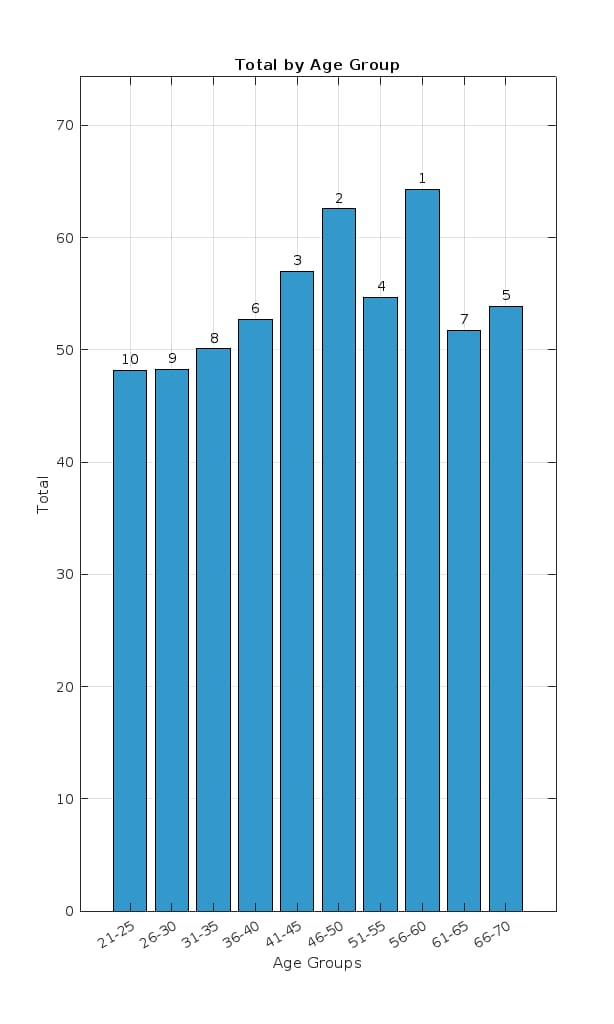
\includegraphics[width=0.7\linewidth,height=0.7\linewidth]{matlab_1.jpg}
\end{figure}
\newpage
\subsubsection{TOPSIS MATLAB CODING:}
\hspace{1em}Utilizing the MATLAB language, a 2-Dimension graph is created to visualize the people age group in connection to the ranking using TOPSIS method’s MCDM process. The MATLAB code given below is used to plot the graph to show the age distribution of diabetic people who are susceptible to emerging viral threats. For the average of people age and rank is taken as input. \\
\begin{lstlisting}[language= MATLAB]
% Data
age_groups = {'21-25', '26-30', '31-35', '36-40', '41-45',
              '46-50', '51-55', '56-60', '61-65', '66-70'};
total_values = [0.77037, 0.81719, 0.71580, 0.73605, 0.72118, 
                0.79352, 0.70796, 0.73897, 0.74803, 0.77177];
rankings = [4, 1, 9, 7, 8, 2, 10, 6, 5, 3];
% Create the bar graph
figure;
bar(total_values, 'b');
% Set the x-tick labels
set(gca, 'XTickLabel', age_groups);
% Title and labels
title('Total Values by Age Group with Rankings');
xlabel('Age Group');
ylabel('Total');
% Display rankings on the bars
for i = 1:length(total_values)
    text(i, total_values(i) + 0.02, num2str(rankings(i)), 'HorizontalAlignment', 'center');
end
% Display grid
grid on;
% Show the figure
hold off;

\end{lstlisting}
\begin{figure}
\begin{center}
    \textbf{OUTPUT}
\end{center}
    \centering
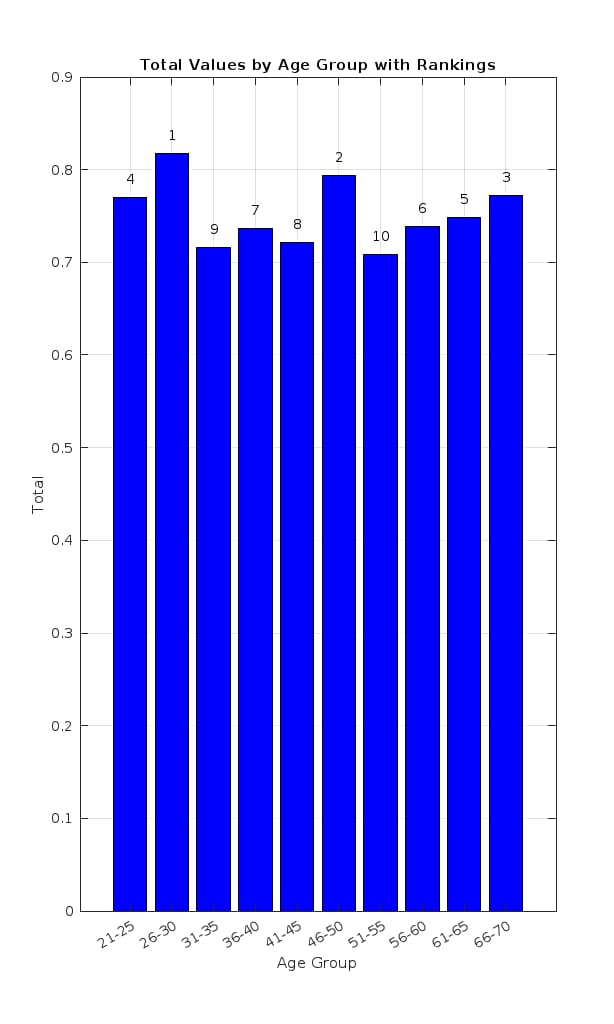
\includegraphics[width=0.7\linewidth,height=0.7\linewidth]{matlab_2.jpg}
\end{figure}

\subsection{COMPARISION OF SAW AND FUZZY TOPSIS}
\begin{enumerate}
    \item \textbf{Methodology:}
    \begin{itemize}
        \item \textbf{SAW :} This method aggregates scores of alternatives across multiple criteria by summing the weighted normalized scores. It is straightforward and easy to implement.

        \item \textbf{Fuzzy TOPSIS :} This method evaluates alternatives based on their distance from an ideal solution. It incorporates fuzzy logic to handle uncertainty and imprecision in data.

        
    \end{itemize}

    \item \textbf{Handling Uncertainty:}
    \begin{itemize}
        \item \textbf{SAW: } While it can use fuzzy numbers, it generally requires precise values for the decision matrix, making it less effective in environments with high uncertainty.

        \item \textbf{Fuzzy TOPSIS: } Specifically designed to manage fuzzy data, it effectively incorporates uncertainty, making it more suitable for applications where data may be imprecise, such as predicting diabetic vulnerability.    
 
    \end{itemize}


    \item \textbf{Decision Criteria:}
    \begin{itemize}
        \item \textbf{SAW: } Requires clearly defined criteria and works well when these criteria are independent. It may struggle with interrelated criteria..

        \item \textbf{Fuzzy TOPSIS: } Can handle correlated criteria more efficiently by comparing the distance to both the ideal and negative-ideal solutions, allowing for more nuanced decision-making.  
 
    \end{itemize}

     \item \textbf{Application Suitability:}
    \begin{itemize}
        \item \textbf{SAW: } Best suited for simpler problems with well-defined metrics. It may provide quick results but can overlook subtleties in complex scenarios.

        \item \textbf{Fuzzy TOPSIS: } More appropriate for complex decision-making situations like assessing diabetic vulnerability where multiple overlapping factors and uncertainties exist.
 
    \end{itemize}
  
\end{enumerate}

\subsection*{Suggested Method for Predicting Diabetic Vulnerability}

\hspace{1em}Given the complexities involved in assessing diabetic vulnerability in the context of emerging viral threats, \textbf{Fuzzy TOPSIS} is recommended. Its ability to manage uncertainty, evaluate interrelated criteria, and provide a robust ranking of alternatives makes it more effective for this application. By incorporating fuzzy logic, the method can accommodate the varying degrees of risk associated with different factors, leading to more accurate and informed decision-making.

\subsection{DEVELOPED PYTHON CODING FOR TOPSIS METHOD}
\textbf{Simple software creation using python:}
\begin{lstlisting}[language= Python]
age=input("Enter the age :")
gulcose=float(input("\nEnter the value of Glucose :"))
blood_pressure=float(input("\nEnter the value of blood pressure :"))
skin_thickness=float(input("\nEnter the value of skin thickness :"))
insulin=float(input("\nEnter the value of insulin :"))
bmi=float(input("\nEnter the value of BMI :"))
diabetes_pedigree_function=float(input("\nEnter the value of Diabetes Pedigree Function :"))


affected_by_diabetes=float(input("\nEnter the value of Affected by diabetes :"))

#lingustic value 
if (0<=affected_by_diabetes<=0.34):
    print(age)
    print("\n",affected_by_diabetes)
    print("\nVery Low")
    l=("Very low")
elif (0<=affected_by_diabetes<=0.44):
    print(age)
    print("\n",affected_by_diabetes)
    print("\nLow")
    l=("Low")
elif (0.45<=affected_by_diabetes<=0.49):
    print(age)
    print("\n",affected_by_diabetes)
    print("\nNormal")
    l=("Normal")
elif (0.50<=affected_by_diabetes<=0.59):
    print(age)
    print("\n",affected_by_diabetes)
    print("\nHigh")
    l=("High")
else :
    print(age)
    print("\n",affected_by_diabetes)
    print("\nVery High")
    l=("Very high")
 
#scale point  
if(l=="Very low"):
    scale_point=1
elif(l=="Low"):
    scale_point=2
elif(l=="Normal"):
    scale_point=3
elif(l=="High"):
    scale_point=4
elif(l=="Very high"):
    scale_point=5
else:
    print("\nInvalid function")

print("\nScale point :",scale_point)
print("\nAffected by diabetics :",affected_by_diabetes)
print("\nlinguistic value of POD :",l)

weightage=0.142
weightage=float(weightage)

print("\nGlucose = Non-Benificial")
print("\nBlood Pressure = Non-Benificial")
print("\nSkin thicness = Non-Benificial")
print("\nInsulin = Benificial")
print("\nScale Point = Non-Benificial")
print("\nBMI = Non-Benificial")
print("\nDiabetes Pedigree Function = Non-Benificial")

max_insulin=float(input("\nEnter the maximum value of insuline :"))
min_glucose=float(input("\nEnter the minimam value of glucose :"))
min_blood_pressure=float(input("\nEnter the minimum value of Blood Pressure :"))
min_skin_thickness=float(input("\nEnter the minimum value of Skin thickness :"))
min_scale_point=float(input("\nEnter the minimum value of Scale point :"))
min_bmi=float(input("\nEnter the minimum value of BMI :"))
min_diabetes=float(input("\nEnter the minimum value of Diabetes pedigree function :"))

a=(min_glucose/gulcose)
a=float(a)
b=(min_blood_pressure/blood_pressure)
b=float(b)
c=(min_skin_thickness/skin_thickness)
c=float(c)
d=(insulin/max_insulin)
d=float(d)
e=(min_scale_point/scale_point)
e=float(e)
f=(min_bmi/bmi)
f=float(f)
g=(min_diabetes/diabetes_pedigree_function)
g=float(g)

print("\nAge :",age)
print("\nGlucose :",a)
print("\nBlood pressure :",b)
print("\nSkin thickness :",c)
print("\nInsulin :",d)
print("\nBMI :",f)
print("\nDiabetes prdigree function :",g)
print("\nScale point :",e)

h=(a*weightage)
h=float(h)
i=(b*weightage)
i=float(i)
j=(c*weightage)
j=float(j)
k=(d*weightage)
k=float(k)
m=(e*weightage)
m=float(m)
n=(f*weightage)
n=float(n)
o=(g*weightage)
o=float(o)

print("\nAge :",age)
print("\nGlucose :",h)
print("\nBlood pressure :",i)
print("\nSkin thickness :",j)
print("\nInsulin :",k)
print("\nBMI :",n)
print("\nDiabetes prdigree function :",o)
print("\nScal_point:",m)

total=(h+i+j+k+m+n+o)
total=float(total)

print("\n",age)
print("Total:",total)
\end{lstlisting}
\newpage

\textbf{Output:}

\begin{figure}[h!]
    \centering
    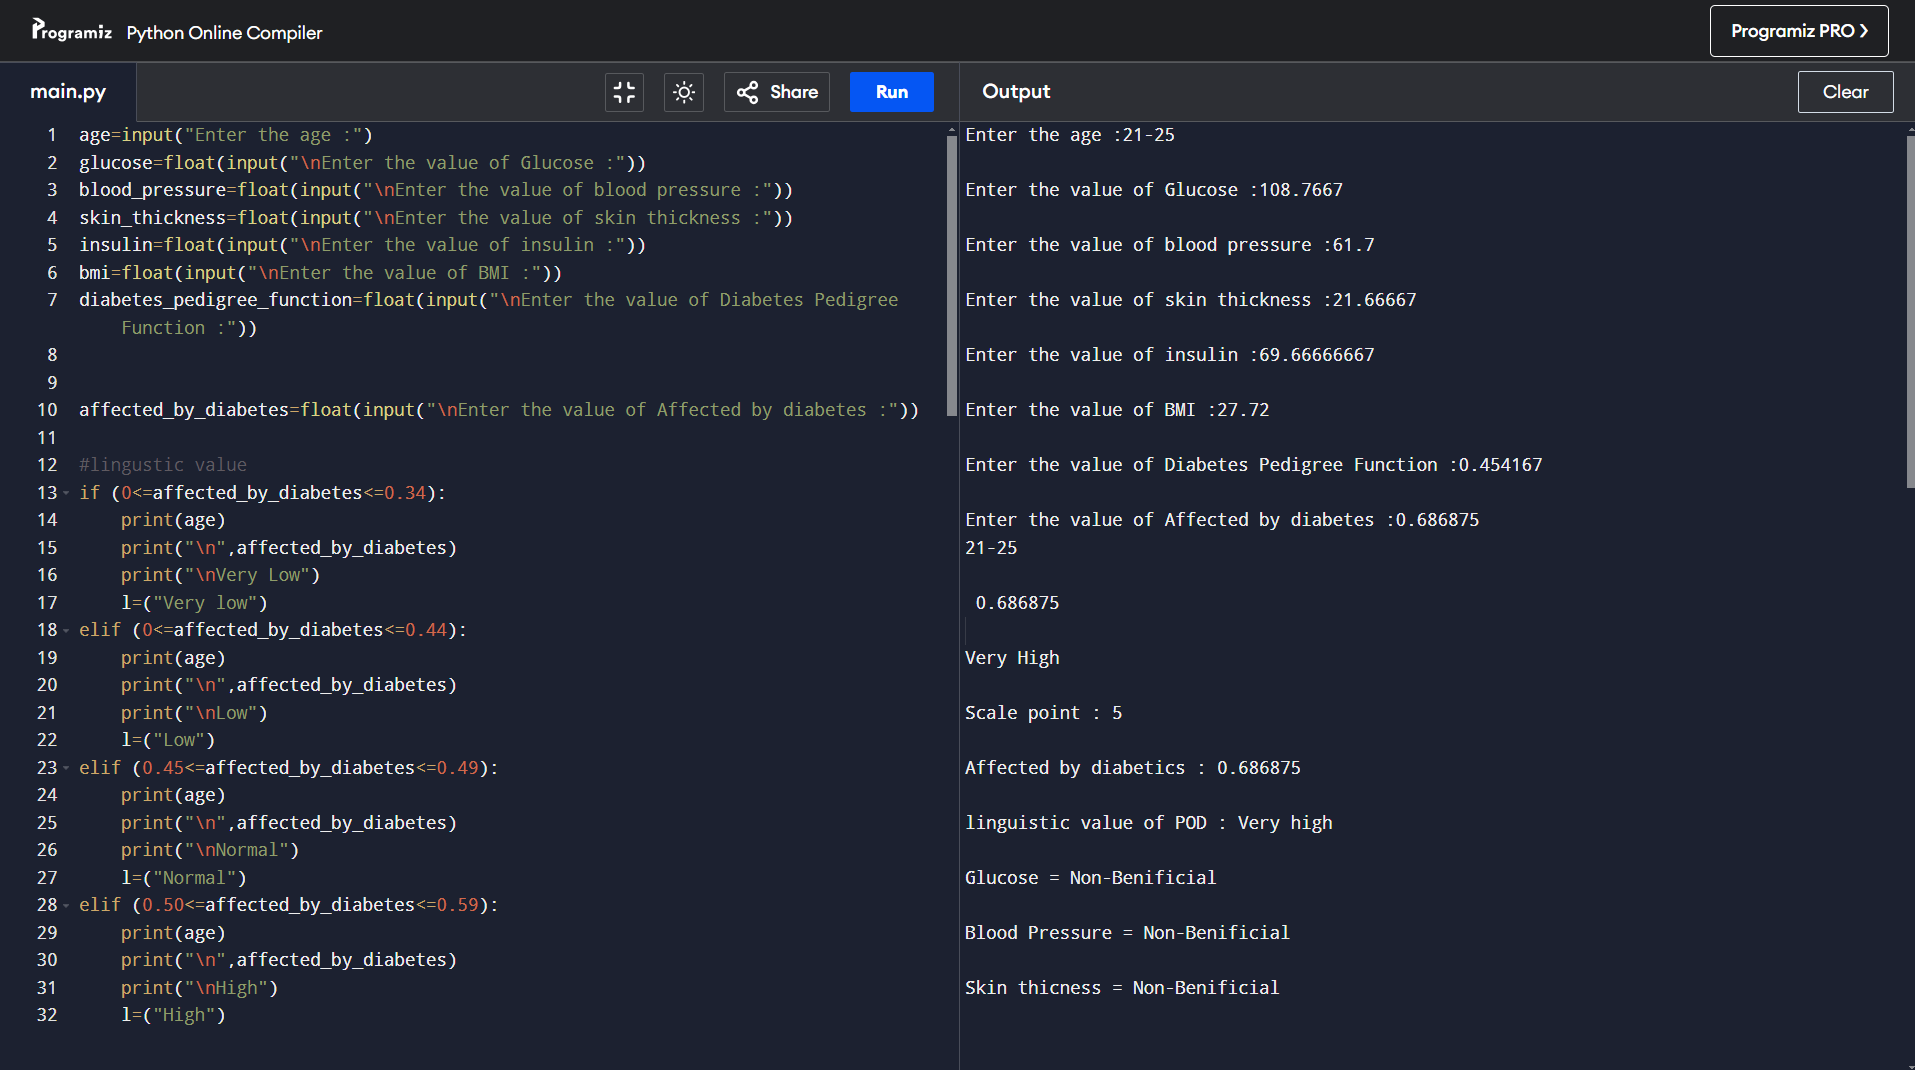
\includegraphics[width=\textwidth]{py_1.png}
    \caption{}
\end{figure}

\begin{figure}[h!]
    \centering
    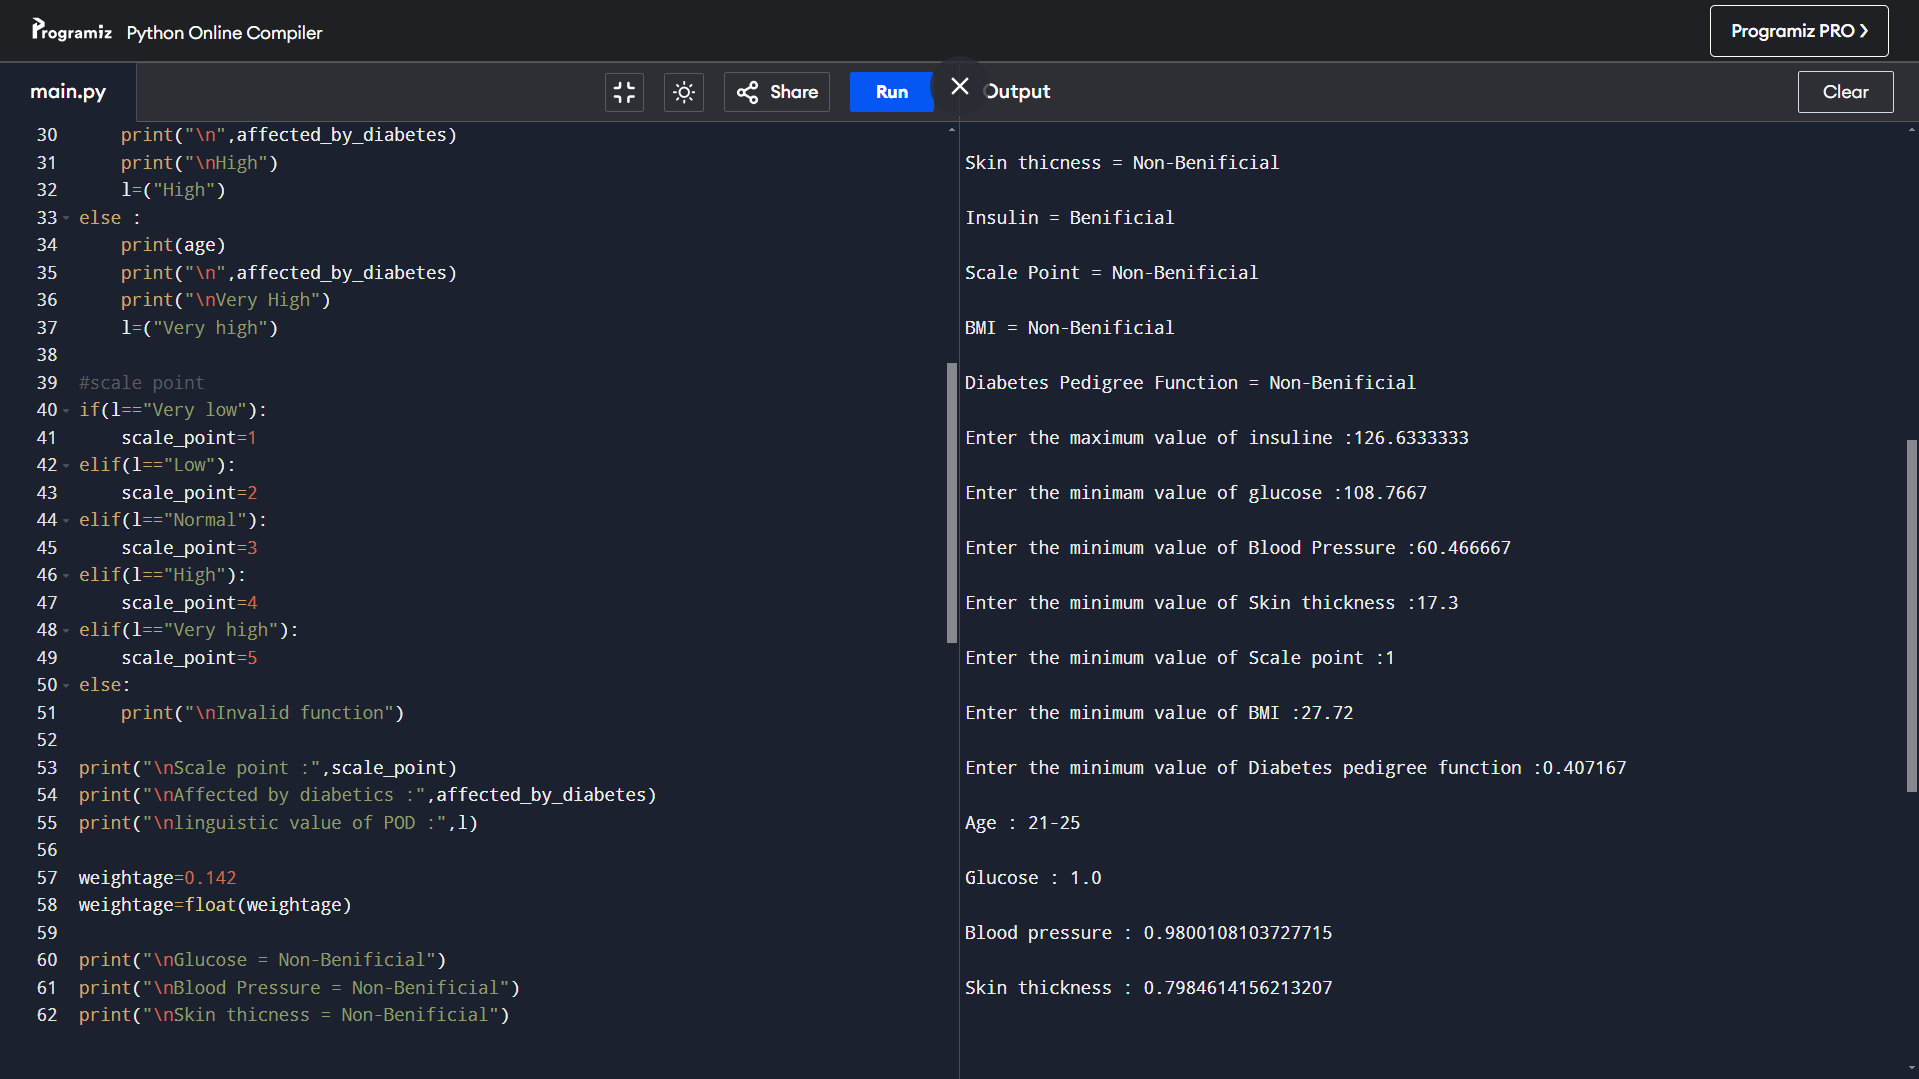
\includegraphics[width=\textwidth]{py_2.png}
    \caption{}
\end{figure}

\newpage

\begin{figure}[h!]
    \centering
    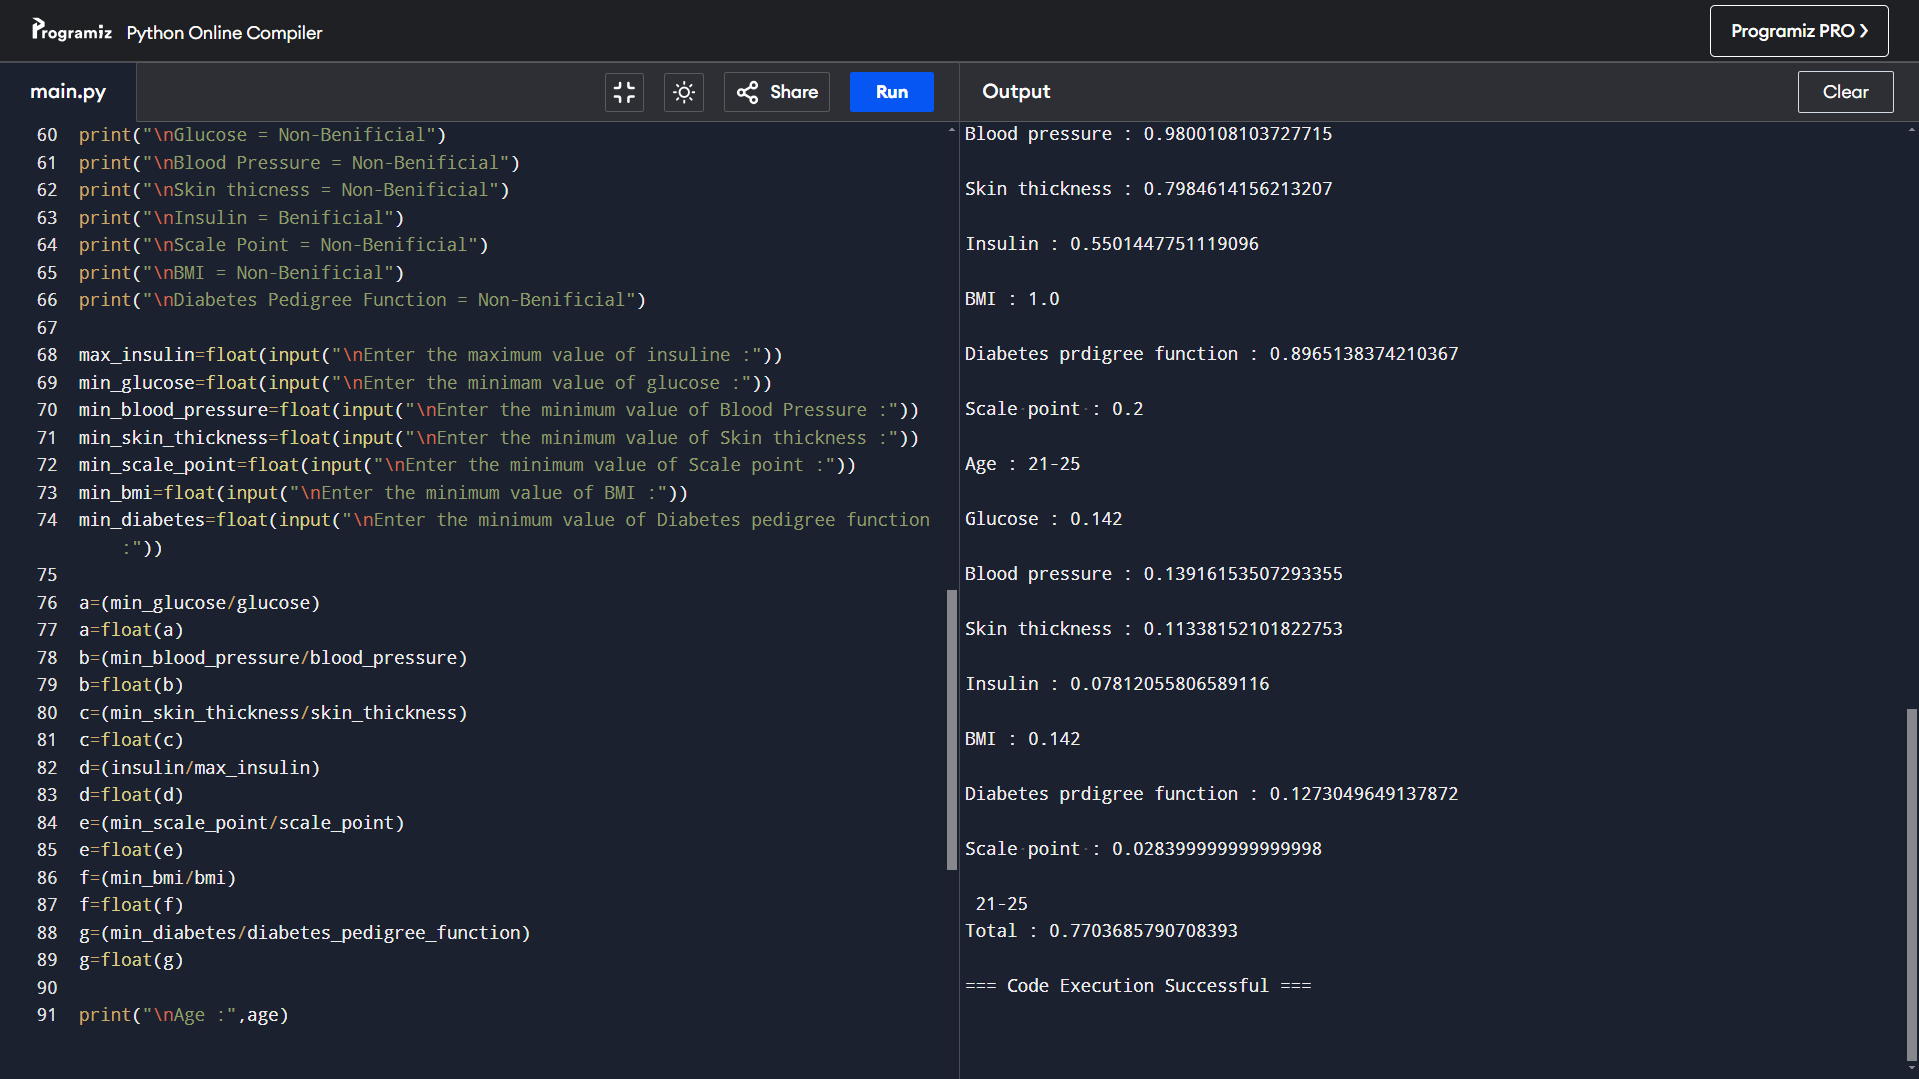
\includegraphics[width=\textwidth]{py_3.png}
    \caption{}
\end{figure}

\begin{figure}[h!]
    \centering
    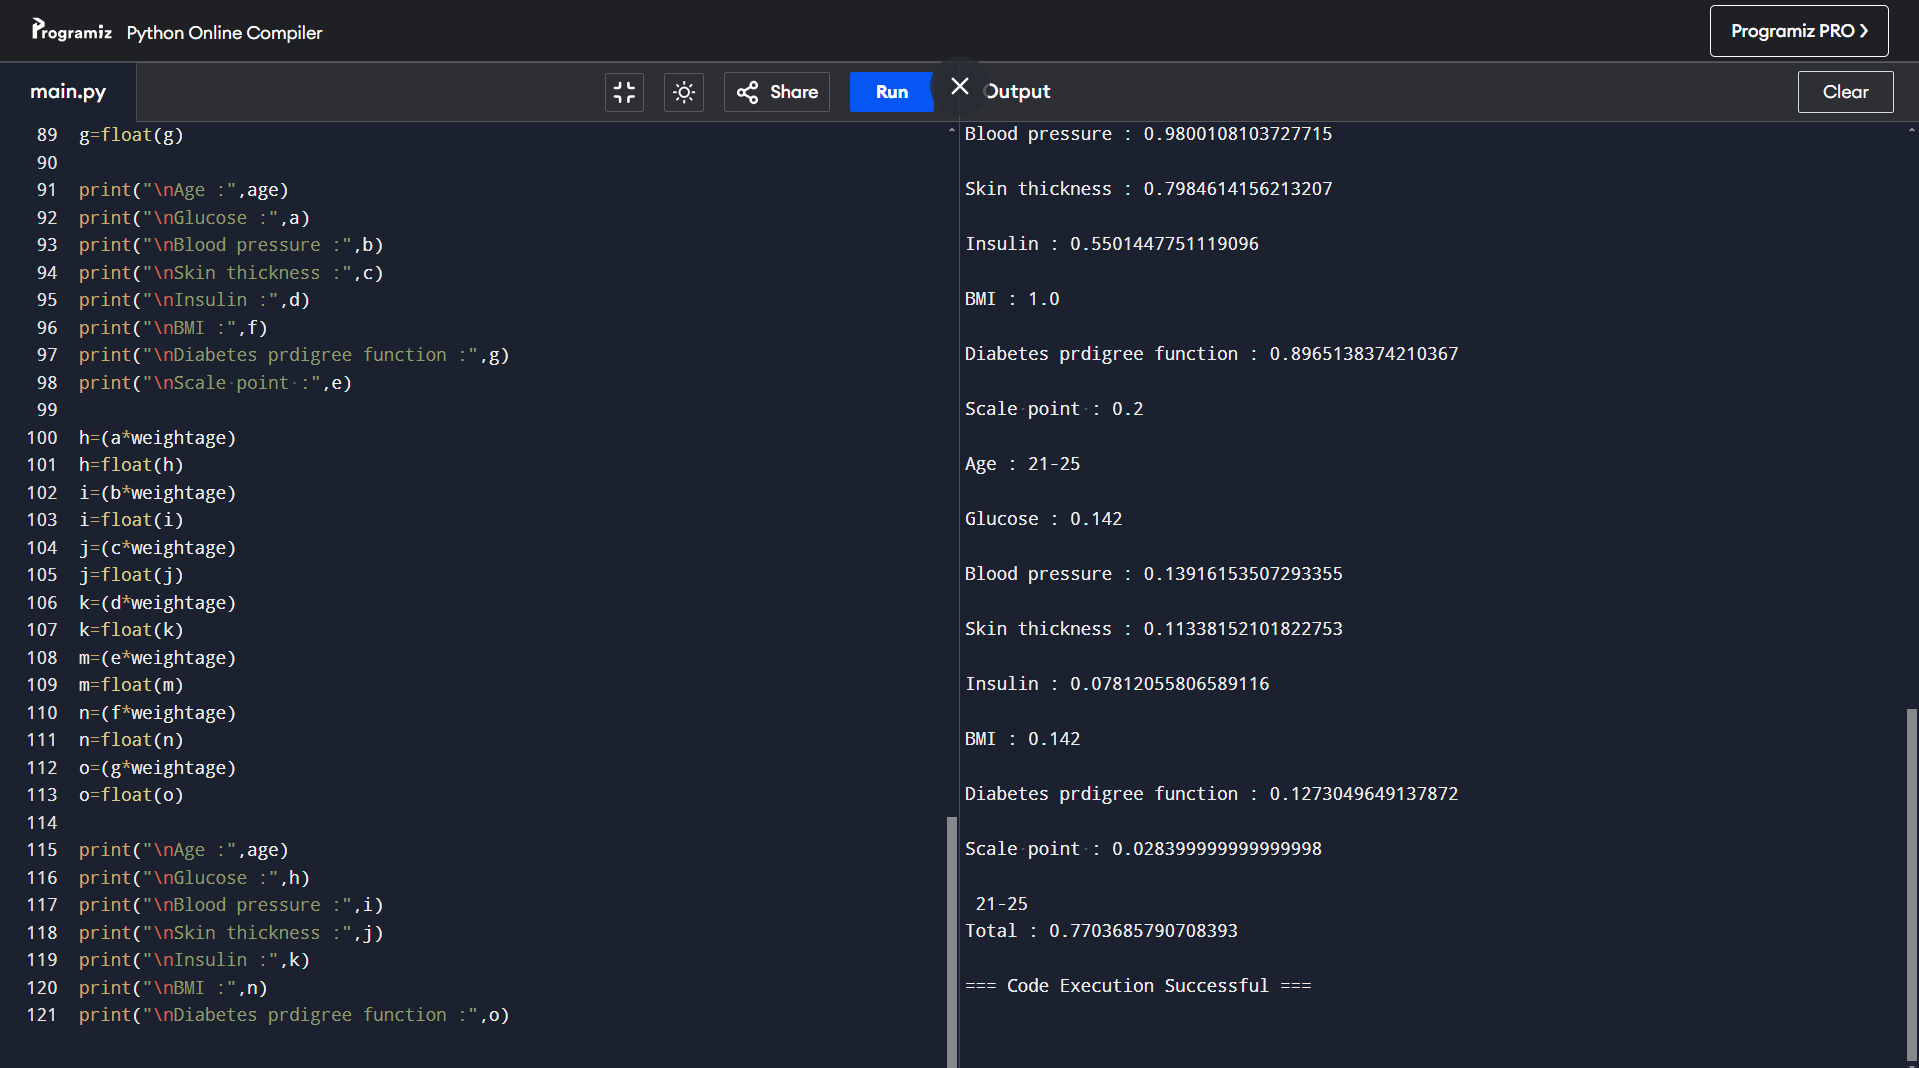
\includegraphics[width=\textwidth]{py_4.png}
    \caption{}
\end{figure}

\begin{figure}[h!]
    \centering
    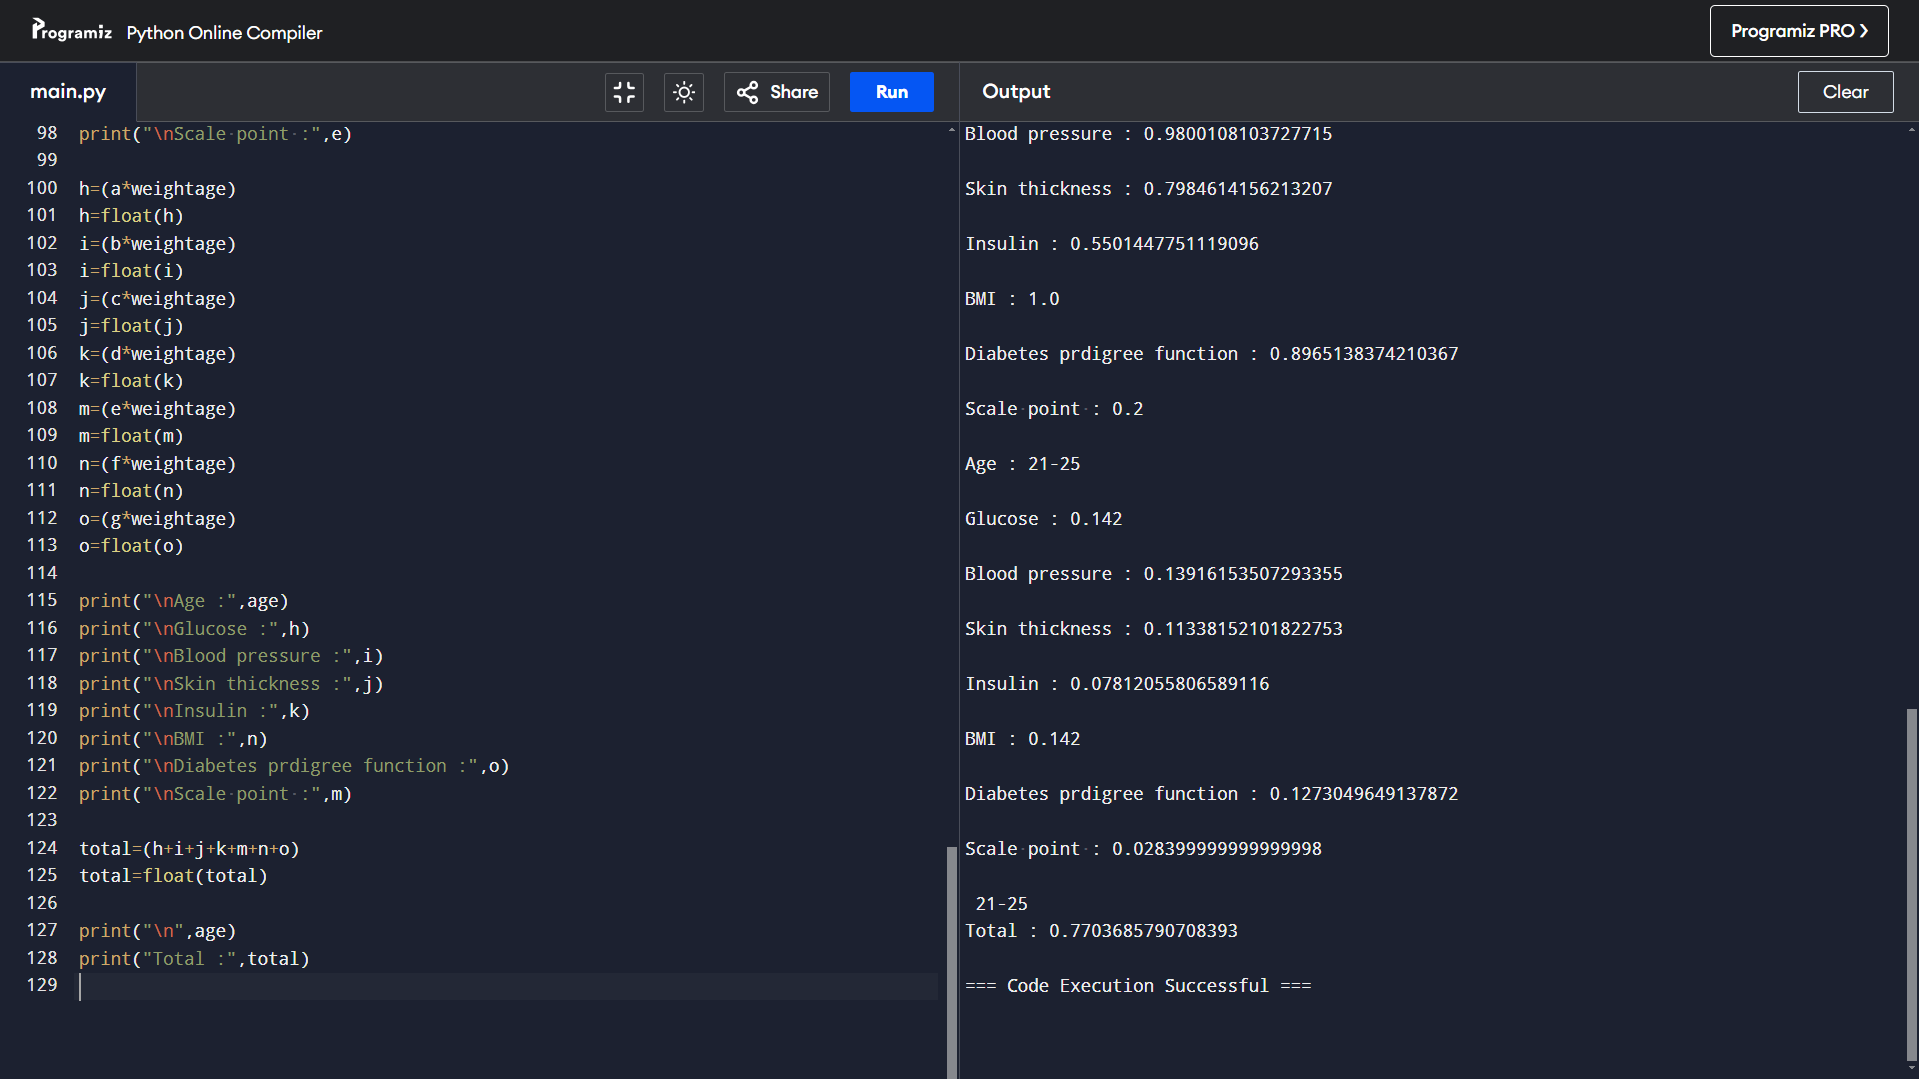
\includegraphics[width=\textwidth]{py_5.png}
    \caption{}
\end{figure}

\newpage
\subsection{SUGGESTIONS FOR CONTROL AND PREVENTION}

\hspace{1em}Preventing viral threats in diabetic patients requires a holistic approach that incorporates dietary choices, lifestyle modifications, and mental well-being practices[3]. Here are some detailed suggestions:

\begin{enumerate}
    \item \textbf{Nutritional Strategies}

    \begin{enumerate}
        \item \textbf{Balanced Diet}

        \begin{itemize}
            \item \textbf{Focus on Whole Foods:} Emphasize vegetables, whole grains, lean proteins, and healthy fats. This helps maintain stable blood sugar levels and overall health.

            \item \textbf{Low Glycemic Index Foods: } Choose foods with a low glycemic index (e.g., legumes, nuts, and most vegetables) to prevent spikes in blood sugar.

            \item \textbf{Adequate Hydration:} Drink plenty of water. Staying hydrated helps the immune system function properly.
            
        \end{itemize}

        \item \textbf{Nutritional Supplements}

        \begin{itemize}
            \item \textbf{Vitamins and Minerals: }Consider supplements like vitamin C, vitamin D, and zinc, which can boost immune function. Consult a healthcare provider before starting any new supplements.


            \item \textbf{Probiotics:} Foods rich in probiotics (like yogurt and fermented vegetables) may enhance gut health, which plays a role in immune response.
            
        \end{itemize}
        
    \end{enumerate}

    \item \textbf{Regular Physical Activity}

    \begin{itemize}

        \item \textbf{Exercise Routine: }Engage in regular physical activity such as walking, cycling, or swimming for at least 150 minutes a week. Exercise helps control blood sugar and enhances immune function.

        \item \textbf{Strength Training:} Incorporate resistance training 2-3 times a week to improve muscle mass and insulin sensitivity.
 
    \end{itemize}

    \item \textbf{Stress Management and Mental Well-being}

    \begin{enumerate}
        \item \textbf{Meditation and Mindfulness}

        \begin{itemize}

        \item \textbf{Daily Meditation: }Practicing mindfulness meditation for 10-20 minutes daily can reduce stress and improve mental clarity, which is beneficial for diabetes management.

        \item \textbf{Deep Breathing Exercises: }  Engage in deep breathing exercises to promote relaxation and reduce anxiety, which can impact blood sugar levels..
     
        \end{itemize}

        \item \textbf{Yoga and Tai Chi}

        \begin{itemize}
            \item \textbf{Gentle Movement Practices: }Incorporate yoga or tai chi into your routine. These practices help reduce stress, improve flexibility, and can aid in blood sugar control.
        \end{itemize}
        
    \end{enumerate}

    \item \textbf{Sleep Hygiene}

     \begin{itemize}

        \item \textbf{Prioritize Sleep: }Aim for 7-9 hours of quality sleep per night. Poor sleep can negatively affect blood sugar levels and immune function.

        \item \textbf{Sleep Routine:  }Maintain a consistent sleep schedule and create a restful environment by minimizing light and noise.
     
        \end{itemize}

        \item \textbf{Preventive Healthcare Measures}

        \begin{itemize}

        \item \textbf{Regular Check-ups:} Schedule routine appointments with healthcare providers to monitor blood sugar levels and overall health.

        \item \textbf{Vaccinations:  }Stay updated on vaccinations, including flu and pneumonia vaccines, which are crucial for diabetic patients.
     
        \end{itemize}

        \item \textbf{Hygiene Practices}

        \begin{itemize}

        \item \textbf{Hand washing: } Practice good hand hygiene by washing hands frequently, especially before meals and after being in public places.

        \item \textbf{Avoiding Crowded Places: } During outbreaks, limit exposure to crowded areas to reduce the risk of infection.
     
        \end{itemize}

        \item \textbf{Educating and Empowering Patients}

        \begin{itemize}

        \item \textbf{Awareness Programs: } Participate in educational workshops or webinars that focus on diabetes management and viral prevention strategies.

        \item \textbf{Support Groups: } Engage in community support groups to share experiences and strategies with other diabetic patients.
     
        \end{itemize}

    \item \textbf{Healthy Snacking}

    \begin{itemize}

        \item \textbf{Smart Snack Choices: }Opt for healthy snacks like nuts, seeds, or cut vegetables. Avoid high-sugar snacks that can cause blood sugar spikes and weaken the immune system.
     
        \end{itemize}

\end{enumerate}


\newpage
\addcontentsline{toc}{section}{CONCLUSION}  
\begin{center}
    \section*{CONCLUSION}
\end{center}
\noindent
\hspace{2em}This project demonstrates the effectiveness of integrating SAW and Fuzzy TOPSIS methodologies to assess the vulnerability of specific age groups to diabetes in the context of emerging viral threats. By analyzing real-time health data, critical metrics influencing susceptibility were identified, enhancing decision-making accuracy in public health contexts. The comparative analysis revealed the respective strengths of these techniques, with Fuzzy TOPSIS emerging as the superior method for this type of analysis.\\

\hspace{1em}Further the development of software using Python code has significantly expedited the generation of results, enabling swift predictions. This project not only contributes to the field of public health but also offers a robust framework for decision-making across diverse sectors, emphasizing the far-reaching impact of interdisciplinary approaches in addressing contemporary challenges.

\newpage
\addcontentsline{toc}{section}{REFERENCES}  % For article class
\begin{thebibliography}{10}
\bibitem{}
Abdullah L.,
\textit{Fuzzy multi criteria decision making and its applications: A brief review of category}, Procedia - Social and Behavioral, Sciences 2013; 97: 131–136.
\bibitem{}
Akhter, M., 
\textit{Enhancing Multi-Criteria Decision Making Using Fuzzy TOPSIS in Sustainable Energy Planning},
Journal of Cleaner Production, 2021.

\bibitem{}
American Diabetes Association,
\textit{Standards of Medical Care in Diabetes – 2024}.
American Diabetes Association, January 2024, 45-68.
\bibitem{}
Bagh Ali,
\textit{Generalized Fuzzy TOPSIS to Solve Multi-Criteria Decision-Making Problems}, Journal of new theory 2020, 44-54.

\bibitem{}
Chen C.T., 
\textit{Extensions of The TOPSIS for Group Decision-Making under Fuzzy Environment}, Fuzzy Sets and Systems 114(1) (2020) 1-9.
\bibitem{}
Chen S. M., 
\textit{Fuzzy sets and fuzzy logic: A historical perspective}.
IEEE, 1996, 1-6.
\bibitem{}
Deveci, M., 
\textit{Evaluation of Energy Economic Optimization Models Using Multi-Criteria Decision-Making Approach}.
Energy Reports, 2024.

\bibitem{}
Hamed Taherdoost, 
\textit{Analysis of Simple Additive Weighting Method (SAW) as a MultiAttribute Decision-Making Technique: A Step-by-Step Guide}.
Journal of Management Science \& Engineering Research, Volume 6, March 2023.

\bibitem{}
Hwang, C. L., \& Yoon, K., 
\textit{Multiple Attribute Decision Making: Methods and Applications}.
Springer-Verlag, 1981, 58-61, 99-116.
\bibitem{}
Kumar, A., \& Kaur, M., 
\textit{A Ranking Approach for Intuitionistic Fuzzy Numbers and its Application}.
International Journal of Fuzzy Logic and Intelligent Systems, 2013.

\bibitem{}
Lavanya, P., 
\textit{Multiple Attribute Decision Making: Methods and Applications}.
Springer-Verlag, 1981, 58-61.

\bibitem{}
Lavanya P,
\textit{Various Fuzzy Number and their various ranking approaches},  International Journal of Advanced Research in Computer Science and Software Engineering in 2017.
\bibitem{}
Ludmila Dymova, 
\textit{An approach to generalization of fuzzy TOPSIS method}.
Elsevier publication, 2013.

\bibitem{}
Lutz, M., 
\textit{Learning Python}.
O'Reilly Media, 5th Edition, 2013, 1-30, 100-120.

\bibitem{}
Mahmodi Nejad, A., \& Mashinchi, M., 
\textit{Ranking Fuzzy Numbers Based on the Areas on the Left and the Right Sides of Fuzzy Numbers}.
Fuzzy Sets and Systems, 2010.

\bibitem{}
McCance, 
\textit{Diabetes: A Comprehensive Guide}.
Wiley-Blackwell, 3rd edition, 2018, 15-45.

\bibitem{}
Mundada, R. G., 
\textit{Design Of A Model For Multistage Classification Of Diabetic Retinopathy And Glaucoma}.
Expert Systems with Applications, 2024.
\bibitem{}
Park .J.H.,  \textit{Extension of the TOPSIS method for decision making problems under interval-valued intuitionistic fuzzy environment}, Applied Mathematical Modelling 2011; 35: 2544–2556.
\bibitem{}
Penso Pereira, A., 
\textit{The Use Of Social Simulation Modelling To Understand Adherence To Diabetic Retinopathy Screening Programs}.
Journal of Medical Systems, 2024.

\bibitem{}
 Peter I. Kattan
\textit{MATLAB for Beginners: A Gentle Approach}.
Petra Books, 2008.

\bibitem{}
Ross, T. J.,  
\textit{Fuzzy Logic with Engineering Applications}.
Wiley, 3rd edition, 2010, 50-75.

\bibitem{}
S. Santhosh,  
\textit{Fuzzy TOPSIS Approach in Identification of Age Group in Women with Diabetes}.
ECB Publications, 2013.

\bibitem{}
Simonovic, S. P.,  
\textit{Fuzzy Set Ranking Methods and Multiple Expert Decision Making}.
Journal of Water Resources Planning and Management, 2001.

\bibitem{}
Singh, R., 
\textit{Fuzzy TOPSIS-Based Approach For Supplier Selection In Supply Chain Management}.
Journal of Supply Chain Management, 2020.

\bibitem{}
Simic, V.,  
\textit{Various Distance Between Generalized Diophantine Fuzzy Sets Using Multiple Criteria Decision Making And Their Real Life Applications}.
Journal of Computational and Applied Mathematics, 2024.

\bibitem{}
Zadeh, H., 
\textit{A Comparative Study Of Fuzzy TOPSIS And Fuzzy AHP For Multi-Criteria Decision Making}.
International Journal of Information Technology \& Decision Making, 2022.

\bibitem{}
Zhang, L.,  
\textit{Integrating Fuzzy TOPSIS and Genetic Algorithms for Multi-Criteria Decision Making}.
Soft Computing, 2019.

\end{thebibliography}

\end{document}
